\documentclass{beamer}
    \usepackage[utf8]{inputenc}
    \usepackage[T1]{fontenc}
    \usepackage[greek,english]{babel}
    \usepackage{bookmark}
    \usepackage{mathtools}
    \usepackage[compatibility,nofetsolderdot,nooldvoltagedirection,european,betterproportions]{circuitikz}
    \usepackage{tikz}
    \usepackage{pgf}
    \usepackage{pgfplots}
    \usepackage{listings}
    \usepackage{ifthen}
    \usepackage{algorithm}% http://ctan.org/pkg/algorithms
    \usepackage{algpseudocode}% http://ctan.org/pkg/algorithmicx

    \usetikzlibrary{positioning, arrows, patterns}

    \usetheme{Berlin}
    \setbeamertemplate{footline}{}
    \setbeamertemplate{headline}{}
    \setbeamertemplate{theorems}[ams style]
    \setbeamertemplate{caption}[numbered]
    % \setbeamercolor{normal text}{bg=gray!5}
    \usecolortheme{lily}
    \usefonttheme{professionalfonts}
    \beamertemplatenavigationsymbolsempty

    \title{Parallel-in-Time Integration in Circuit Simulation}
    \author[F. Madge]{Fabio Madge}
    % \institute{Technische Universität München}
    \date[24.09.19]{24. September 2019}

\begin{document}

    \maketitle

    \begin{frame}
    \setcounter{tocdepth}{1}
    \tableofcontents[pausesections]
    \end{frame}

    \AtBeginSection[]
    {
    \begin{frame}
    \setcounter{tocdepth}{2}
    \tableofcontents[currentsection,hideothersubsections]
    \end{frame}
    }

    \AtBeginSubsection[]
    {
    \begin{frame}
    \setcounter{tocdepth}{2}
    \tableofcontents[currentsection,
            currentsubsection,
            subsectionstyle=show/shaded/hide]
    \end{frame}
    }

    \section{Introduction}
    \subsection{Circuit Simulation}
\begin{frame}
\frametitle{Circuit (Example)}
\begin{figure}[ht]
    \centering\scalebox{1.5}{
        \begin{circuitikz}[scale=1.5]
            \draw (0,0) node[ground] {} to ++(0,1)
        -- ++(0,0) to[*R=$R$,a=$1\,\Omega$,-*] ++(2,0) node[above]{$1$}
        -- ++(0,0) to[*C=$C$,a=$100\,\mathrm{nF}$] ++(2,0)
        -- ++(0,0) to ++(0,-1) node[ground] {};
% \draw (3,0) to[R=1,i>_=1, o-*] (6,0);
        \end{circuitikz}}
    \caption{Loaded capacitor}
\label{fig:cap}
\end{figure}
\begin{itemize}
    \item Specified in a netlist file
    \item Can contain \(>\!10^6\) devices
\end{itemize}
% Electric current \(I\)? E.g \(i_1\) at node 1.\\
% Electric potential \(U\)? E.g \(u_1\) at node 1.
\end{frame}

\begin{frame}
\frametitle{Simulation}
\begin{block}{Questions}
    \begin{itemize}
        \item Electric current \(I\)? E.g \(i_R\) current through device R.
        \item Electric potential \(U\)? E.g \(u_1\) potential at node 1.
        \item Behavior over time? Transient response?
    \end{itemize}
\end{block}
\begin{block}{Solution}
    \begin{enumerate}
        \item Find a stable oparating point (.OP)
        \item Find trajectory of \(I\) and \(U\) over time (.TRAN)
    \end{enumerate}
\end{block}
\end{frame}

\begin{frame}
    \centering
    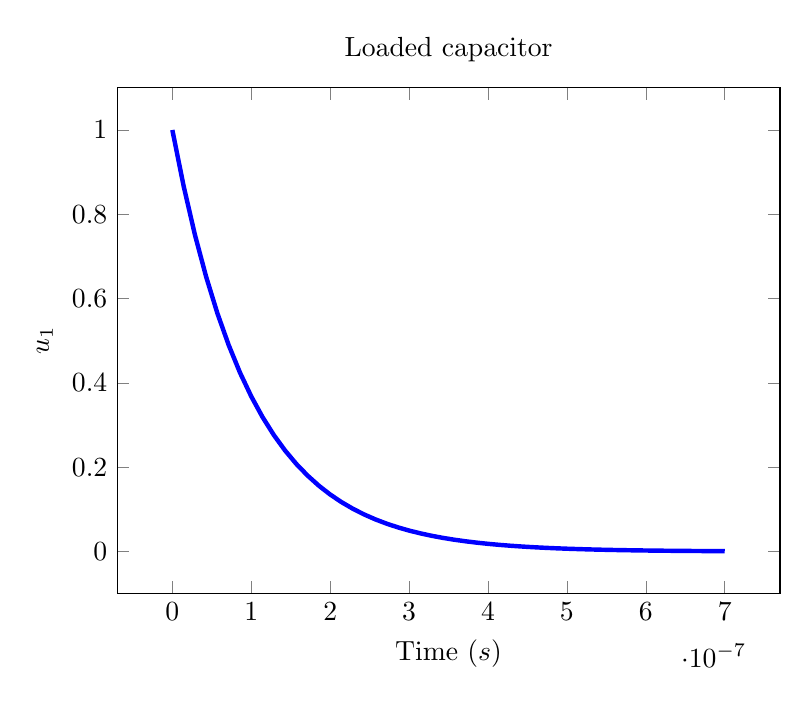
\begin{tikzpicture}
        \begin{axis}[
            samples=50,
            title=Loaded capacitor,
            xlabel={Time $(s)$},
            ylabel={$u_1$},
            width=10cm,
            height=8cm]
          \addplot[blue, ultra thick,domain=0:7e-7] ({x},{exp(-(x/(1e-7)))});
        \end{axis}
    \end{tikzpicture}
\end{frame}

\begin{frame}
\frametitle{Modified Nodal Analysis\footfullcite{Gunther:2005}}
\begin{itemize}[<+->]
    \item Every element has a model:
        \begin{itemize}
            \item{Resistor: \(I = G \cdot U,\quad G=\frac{1}{R}\)
            \begin{description}[]
                \item[\(G\)]<.->  Conductance
            \end{description}}
            \item Capacitor: \(I = C \cdot \dot{U}\)
            \begin{description}[]
                \item[\(C\)]<.-> Capacity
            \end{description}
            \item \dots
        \end{itemize}
    \item Abstraction of the circuit as a graph \(G = (V,E)\)
    \begin{description}[]
        \item[\(V\)]<.-> Vertex
        \item[\(E\)]<.-> Edge
    \end{description}
    \item Kirchhoff's current law: \(\forall v \in V. \sum_{j \in E(v)} i_{j} = 0\)
    \begin{description}[]
        \item[\(E(v)\)] Edges connected to Vertex v
    \end{description}
\end{itemize}
\end{frame}

\begin{frame}
\frametitle{Example}
KCL: \(\forall v \in V. \sum_{j \in E(v)} i_{j} = 0\); Resistor: \(I = G \cdot U\); Cap: \(I = C \cdot \dot{U}\)
\begin{figure}[ht]
    \centering
        \begin{circuitikz}
            \draw (0,0) node[ground] {} to ++(0,1)
        -- ++(0,0) to[*R=$R$,a=$1\,\Omega$,-*] ++(2,0) node[above]{$1$}
        -- ++(0,0) to[*C=$C$,a=$100\,\mathrm{nF}$] ++(2,0)
        -- ++(0,0) to ++(0,-1) node[ground] {};
% \draw (3,0) to[R=1,i>_=1, o-*] (6,0);
        \end{circuitikz}
    \caption{Loaded capacitor}
\label{fig:cap}
\end{figure}
\pause
\begin{enumerate}[<+->]
    \item Concrete equation for this example:\\
        \(C\dot{u}_1 + Gu_1 = 0\)
    \item Generalization for bigger circuits:\\
        \(\mathbf{C}(\vec{x}) \cdot \dot{\vec{x}} + \mathbf{G} \vec{x} = \vec{s}(t)\)
    \item Application of generalized discretization (more later):\\
        \(\mathbf{C}(\vec{x}) \cdot (\alpha \vec{x} + \beta) + \mathbf{G} \vec{x} = \vec{s}(t)\)
    \item Prepare for Newton's method:\\
        \(\mathbf{C}(\vec{x}) \cdot (\alpha \vec{x} + \beta) + \mathbf{G} \vec{x} - \vec{s}(t)= 0\)
\end{enumerate}
\end{frame}

\begin{frame}
\frametitle{.TRAN}
\begin{itemize}
    \item .OP
    \item For every time step \(t_i \in \left(t_0, T\right]\):
    \begin{itemize}
        \item While not sufficiently close to solution:
        \begin{itemize}
            \item Calc \(\alpha, \beta\)
            \item Evaluate models
            \item Assemble problem
            \item Use linear solver
            \item Apply correction
        \end{itemize}
    \end{itemize}
\end{itemize}
\end{frame}


\subsection{Parallel Numerical Integration}
\begin{frame}
\frametitle{Problem: Inital Value Problem}
\begin{equation*}
y'(t) = f(t,y(t)), \quad y(t_0) = y_0.
\end{equation*}
\end{frame}

\begin{frame}
\frametitle{Solution*: Numerics \(\rightarrow\) discretization}
\begin{exampleblock}{Implicit Euler}
\begin{equation*}
y_{n+1} = y_n + hf(t_{n+1},y_{n+1})
\end{equation*}
\begin{equation*}
    f(t_{n+1},y_{n+1}) = \frac{y_{n+1} - y_n}{h}
    \end{equation*}
\begin{description}[]
    \item[\(h\)] stepsize
\end{description}
\pause
\begin{block}{Generalized}
    \begin{equation*}
        \dot{y}_{n+1} = \alpha \cdot y_{n+1} + \beta
    \end{equation*}
    \begin{equation*}
        \alpha = \frac{1}{h}\quad\beta = - \frac{y_n}{h}
    \end{equation*}
\end{block}
\end{exampleblock}
\pause
\begin{alertblock}{Strictly sequential}
Problematic for parallelization
\end{alertblock}
\end{frame}



    \section{Algorithm: Parareal}
    \subsection{Corrections}

\begin{frame}
\begin{equation*}
y_{j+1}^{k+1} = \mathcal{G}\!\!\left(y_j^{k+1}, t_j, t_{j+1}\right) + \mathcal{F}\!\!\left(y_j^k, t_j, t_{j+1}\right) - \mathcal{G}\!\!\left(y_j^k, t_j, t_{j+1}\right)
\end{equation*}
\end{frame}

\begin{frame}
\begin{center}
\includegraphics[width=70mm]{sequence.jpg}
\end{center}
\begin{equation*}
y_{j+1}^{k+1} = \mathcal{G}\!\!\left(y_j^{k+1}, t_j, t_{j+1}\right) + \mathcal{F}\!\!\left(y_j^k, t_j, t_{j+1}\right) - \mathcal{G}\!\!\left(y_j^k, t_j, t_{j+1}\right)
\end{equation*}
\end{frame}

\subsection{Evaluation}

\begin{frame}
\begin{center}
\scalebox{0.65}{\input{plots/kmaxStudy.pgf}}
\end{center}
\end{frame}

\begin{frame}
\begin{center}
\scalebox{0.65}{\input{plots/iterLocalError.pgf}}
\end{center}
\end{frame}



\begin{frame}
\begin{center}
\scalebox{0.65}{\input{plots/iterError.pgf}}
\end{center}
\end{frame}

\begin{frame}
\begin{center}
\scalebox{0.65}{\input{plots/errorDisc.pgf}}
\end{center}
\end{frame}




    \section{Application}
    \subsection{Implementation}

\begin{frame}
\frametitle{tictac}
\begin{itemize}[<+->]
    \item Circuit simulator written in \texttt{C++}
    \item Comes with BE and TR integrators
    \item Limited but sufficient collection of devices
    \item .OP and .TRAN
\end{itemize}
\end{frame}

\begin{frame}
how does it work?
\end{frame}

\subsection{Results}

\begin{frame}
    \begin{figure}[ht]
        \centering
        \scalebox{0.8}{%% Creator: Matplotlib, PGF backend
%%
%% To include the figure in your LaTeX document, write
%%   \input{<filename>.pgf}
%%
%% Make sure the required packages are loaded in your preamble
%%   \usepackage{pgf}
%%
%% Figures using additional raster images can only be included by \input if
%% they are in the same directory as the main LaTeX file. For loading figures
%% from other directories you can use the `import` package
%%   \usepackage{import}
%% and then include the figures with
%%   \import{<path to file>}{<filename>.pgf}
%%
%% Matplotlib used the following preamble
%%   \usepackage{fontspec}
%%   \setmainfont{Times New Roman}
%%   \setsansfont{Lucida Grande}
%%   \setmonofont{Andale Mono}
%%
\begingroup%
\makeatletter%
\begin{pgfpicture}%
\pgfpathrectangle{\pgfpointorigin}{\pgfqpoint{5.000000in}{3.083333in}}%
\pgfusepath{use as bounding box, clip}%
\begin{pgfscope}%
\pgfsetbuttcap%
\pgfsetmiterjoin%
\definecolor{currentfill}{rgb}{1.000000,1.000000,1.000000}%
\pgfsetfillcolor{currentfill}%
\pgfsetlinewidth{0.000000pt}%
\definecolor{currentstroke}{rgb}{1.000000,1.000000,1.000000}%
\pgfsetstrokecolor{currentstroke}%
\pgfsetdash{}{0pt}%
\pgfpathmoveto{\pgfqpoint{0.000000in}{0.000000in}}%
\pgfpathlineto{\pgfqpoint{5.000000in}{0.000000in}}%
\pgfpathlineto{\pgfqpoint{5.000000in}{3.083333in}}%
\pgfpathlineto{\pgfqpoint{0.000000in}{3.083333in}}%
\pgfpathclose%
\pgfusepath{fill}%
\end{pgfscope}%
\begin{pgfscope}%
\pgfsetbuttcap%
\pgfsetmiterjoin%
\definecolor{currentfill}{rgb}{1.000000,1.000000,1.000000}%
\pgfsetfillcolor{currentfill}%
\pgfsetlinewidth{0.000000pt}%
\definecolor{currentstroke}{rgb}{0.000000,0.000000,0.000000}%
\pgfsetstrokecolor{currentstroke}%
\pgfsetstrokeopacity{0.000000}%
\pgfsetdash{}{0pt}%
\pgfpathmoveto{\pgfqpoint{0.467954in}{0.402778in}}%
\pgfpathlineto{\pgfqpoint{4.880181in}{0.402778in}}%
\pgfpathlineto{\pgfqpoint{4.880181in}{3.034722in}}%
\pgfpathlineto{\pgfqpoint{0.467954in}{3.034722in}}%
\pgfpathclose%
\pgfusepath{fill}%
\end{pgfscope}%
\begin{pgfscope}%
\pgfsetbuttcap%
\pgfsetroundjoin%
\definecolor{currentfill}{rgb}{0.000000,0.000000,0.000000}%
\pgfsetfillcolor{currentfill}%
\pgfsetlinewidth{0.803000pt}%
\definecolor{currentstroke}{rgb}{0.000000,0.000000,0.000000}%
\pgfsetstrokecolor{currentstroke}%
\pgfsetdash{}{0pt}%
\pgfsys@defobject{currentmarker}{\pgfqpoint{0.000000in}{-0.048611in}}{\pgfqpoint{0.000000in}{0.000000in}}{%
\pgfpathmoveto{\pgfqpoint{0.000000in}{0.000000in}}%
\pgfpathlineto{\pgfqpoint{0.000000in}{-0.048611in}}%
\pgfusepath{stroke,fill}%
}%
\begin{pgfscope}%
\pgfsys@transformshift{0.668510in}{0.402778in}%
\pgfsys@useobject{currentmarker}{}%
\end{pgfscope}%
\end{pgfscope}%
\begin{pgfscope}%
\pgftext[x=0.668510in,y=0.305556in,,top]{\rmfamily\fontsize{10.000000}{12.000000}\selectfont \(\displaystyle 0.0000000\)}%
\end{pgfscope}%
\begin{pgfscope}%
\pgfsetbuttcap%
\pgfsetroundjoin%
\definecolor{currentfill}{rgb}{0.000000,0.000000,0.000000}%
\pgfsetfillcolor{currentfill}%
\pgfsetlinewidth{0.803000pt}%
\definecolor{currentstroke}{rgb}{0.000000,0.000000,0.000000}%
\pgfsetstrokecolor{currentstroke}%
\pgfsetdash{}{0pt}%
\pgfsys@defobject{currentmarker}{\pgfqpoint{0.000000in}{-0.048611in}}{\pgfqpoint{0.000000in}{0.000000in}}{%
\pgfpathmoveto{\pgfqpoint{0.000000in}{0.000000in}}%
\pgfpathlineto{\pgfqpoint{0.000000in}{-0.048611in}}%
\pgfusepath{stroke,fill}%
}%
\begin{pgfscope}%
\pgfsys@transformshift{1.470732in}{0.402778in}%
\pgfsys@useobject{currentmarker}{}%
\end{pgfscope}%
\end{pgfscope}%
\begin{pgfscope}%
\pgftext[x=1.470732in,y=0.305556in,,top]{\rmfamily\fontsize{10.000000}{12.000000}\selectfont \(\displaystyle 0.0000002\)}%
\end{pgfscope}%
\begin{pgfscope}%
\pgfsetbuttcap%
\pgfsetroundjoin%
\definecolor{currentfill}{rgb}{0.000000,0.000000,0.000000}%
\pgfsetfillcolor{currentfill}%
\pgfsetlinewidth{0.803000pt}%
\definecolor{currentstroke}{rgb}{0.000000,0.000000,0.000000}%
\pgfsetstrokecolor{currentstroke}%
\pgfsetdash{}{0pt}%
\pgfsys@defobject{currentmarker}{\pgfqpoint{0.000000in}{-0.048611in}}{\pgfqpoint{0.000000in}{0.000000in}}{%
\pgfpathmoveto{\pgfqpoint{0.000000in}{0.000000in}}%
\pgfpathlineto{\pgfqpoint{0.000000in}{-0.048611in}}%
\pgfusepath{stroke,fill}%
}%
\begin{pgfscope}%
\pgfsys@transformshift{2.272955in}{0.402778in}%
\pgfsys@useobject{currentmarker}{}%
\end{pgfscope}%
\end{pgfscope}%
\begin{pgfscope}%
\pgftext[x=2.272955in,y=0.305556in,,top]{\rmfamily\fontsize{10.000000}{12.000000}\selectfont \(\displaystyle 0.0000004\)}%
\end{pgfscope}%
\begin{pgfscope}%
\pgfsetbuttcap%
\pgfsetroundjoin%
\definecolor{currentfill}{rgb}{0.000000,0.000000,0.000000}%
\pgfsetfillcolor{currentfill}%
\pgfsetlinewidth{0.803000pt}%
\definecolor{currentstroke}{rgb}{0.000000,0.000000,0.000000}%
\pgfsetstrokecolor{currentstroke}%
\pgfsetdash{}{0pt}%
\pgfsys@defobject{currentmarker}{\pgfqpoint{0.000000in}{-0.048611in}}{\pgfqpoint{0.000000in}{0.000000in}}{%
\pgfpathmoveto{\pgfqpoint{0.000000in}{0.000000in}}%
\pgfpathlineto{\pgfqpoint{0.000000in}{-0.048611in}}%
\pgfusepath{stroke,fill}%
}%
\begin{pgfscope}%
\pgfsys@transformshift{3.075177in}{0.402778in}%
\pgfsys@useobject{currentmarker}{}%
\end{pgfscope}%
\end{pgfscope}%
\begin{pgfscope}%
\pgftext[x=3.075177in,y=0.305556in,,top]{\rmfamily\fontsize{10.000000}{12.000000}\selectfont \(\displaystyle 0.0000006\)}%
\end{pgfscope}%
\begin{pgfscope}%
\pgfsetbuttcap%
\pgfsetroundjoin%
\definecolor{currentfill}{rgb}{0.000000,0.000000,0.000000}%
\pgfsetfillcolor{currentfill}%
\pgfsetlinewidth{0.803000pt}%
\definecolor{currentstroke}{rgb}{0.000000,0.000000,0.000000}%
\pgfsetstrokecolor{currentstroke}%
\pgfsetdash{}{0pt}%
\pgfsys@defobject{currentmarker}{\pgfqpoint{0.000000in}{-0.048611in}}{\pgfqpoint{0.000000in}{0.000000in}}{%
\pgfpathmoveto{\pgfqpoint{0.000000in}{0.000000in}}%
\pgfpathlineto{\pgfqpoint{0.000000in}{-0.048611in}}%
\pgfusepath{stroke,fill}%
}%
\begin{pgfscope}%
\pgfsys@transformshift{3.877399in}{0.402778in}%
\pgfsys@useobject{currentmarker}{}%
\end{pgfscope}%
\end{pgfscope}%
\begin{pgfscope}%
\pgftext[x=3.877399in,y=0.305556in,,top]{\rmfamily\fontsize{10.000000}{12.000000}\selectfont \(\displaystyle 0.0000008\)}%
\end{pgfscope}%
\begin{pgfscope}%
\pgfsetbuttcap%
\pgfsetroundjoin%
\definecolor{currentfill}{rgb}{0.000000,0.000000,0.000000}%
\pgfsetfillcolor{currentfill}%
\pgfsetlinewidth{0.803000pt}%
\definecolor{currentstroke}{rgb}{0.000000,0.000000,0.000000}%
\pgfsetstrokecolor{currentstroke}%
\pgfsetdash{}{0pt}%
\pgfsys@defobject{currentmarker}{\pgfqpoint{0.000000in}{-0.048611in}}{\pgfqpoint{0.000000in}{0.000000in}}{%
\pgfpathmoveto{\pgfqpoint{0.000000in}{0.000000in}}%
\pgfpathlineto{\pgfqpoint{0.000000in}{-0.048611in}}%
\pgfusepath{stroke,fill}%
}%
\begin{pgfscope}%
\pgfsys@transformshift{4.679621in}{0.402778in}%
\pgfsys@useobject{currentmarker}{}%
\end{pgfscope}%
\end{pgfscope}%
\begin{pgfscope}%
\pgftext[x=4.679621in,y=0.305556in,,top]{\rmfamily\fontsize{10.000000}{12.000000}\selectfont \(\displaystyle 0.0000010\)}%
\end{pgfscope}%
\begin{pgfscope}%
\pgftext[x=2.674068in,y=0.123861in,,top]{\rmfamily\fontsize{10.000000}{12.000000}\selectfont t}%
\end{pgfscope}%
\begin{pgfscope}%
\pgfsetbuttcap%
\pgfsetroundjoin%
\definecolor{currentfill}{rgb}{0.000000,0.000000,0.000000}%
\pgfsetfillcolor{currentfill}%
\pgfsetlinewidth{0.803000pt}%
\definecolor{currentstroke}{rgb}{0.000000,0.000000,0.000000}%
\pgfsetstrokecolor{currentstroke}%
\pgfsetdash{}{0pt}%
\pgfsys@defobject{currentmarker}{\pgfqpoint{-0.048611in}{0.000000in}}{\pgfqpoint{0.000000in}{0.000000in}}{%
\pgfpathmoveto{\pgfqpoint{0.000000in}{0.000000in}}%
\pgfpathlineto{\pgfqpoint{-0.048611in}{0.000000in}}%
\pgfusepath{stroke,fill}%
}%
\begin{pgfscope}%
\pgfsys@transformshift{0.467954in}{0.522303in}%
\pgfsys@useobject{currentmarker}{}%
\end{pgfscope}%
\end{pgfscope}%
\begin{pgfscope}%
\pgftext[x=0.193262in,y=0.474085in,left,base]{\rmfamily\fontsize{10.000000}{12.000000}\selectfont \(\displaystyle 0.0\)}%
\end{pgfscope}%
\begin{pgfscope}%
\pgfsetbuttcap%
\pgfsetroundjoin%
\definecolor{currentfill}{rgb}{0.000000,0.000000,0.000000}%
\pgfsetfillcolor{currentfill}%
\pgfsetlinewidth{0.803000pt}%
\definecolor{currentstroke}{rgb}{0.000000,0.000000,0.000000}%
\pgfsetstrokecolor{currentstroke}%
\pgfsetdash{}{0pt}%
\pgfsys@defobject{currentmarker}{\pgfqpoint{-0.048611in}{0.000000in}}{\pgfqpoint{0.000000in}{0.000000in}}{%
\pgfpathmoveto{\pgfqpoint{0.000000in}{0.000000in}}%
\pgfpathlineto{\pgfqpoint{-0.048611in}{0.000000in}}%
\pgfusepath{stroke,fill}%
}%
\begin{pgfscope}%
\pgfsys@transformshift{0.467954in}{1.000860in}%
\pgfsys@useobject{currentmarker}{}%
\end{pgfscope}%
\end{pgfscope}%
\begin{pgfscope}%
\pgftext[x=0.193262in,y=0.952642in,left,base]{\rmfamily\fontsize{10.000000}{12.000000}\selectfont \(\displaystyle 0.2\)}%
\end{pgfscope}%
\begin{pgfscope}%
\pgfsetbuttcap%
\pgfsetroundjoin%
\definecolor{currentfill}{rgb}{0.000000,0.000000,0.000000}%
\pgfsetfillcolor{currentfill}%
\pgfsetlinewidth{0.803000pt}%
\definecolor{currentstroke}{rgb}{0.000000,0.000000,0.000000}%
\pgfsetstrokecolor{currentstroke}%
\pgfsetdash{}{0pt}%
\pgfsys@defobject{currentmarker}{\pgfqpoint{-0.048611in}{0.000000in}}{\pgfqpoint{0.000000in}{0.000000in}}{%
\pgfpathmoveto{\pgfqpoint{0.000000in}{0.000000in}}%
\pgfpathlineto{\pgfqpoint{-0.048611in}{0.000000in}}%
\pgfusepath{stroke,fill}%
}%
\begin{pgfscope}%
\pgfsys@transformshift{0.467954in}{1.479417in}%
\pgfsys@useobject{currentmarker}{}%
\end{pgfscope}%
\end{pgfscope}%
\begin{pgfscope}%
\pgftext[x=0.193262in,y=1.431199in,left,base]{\rmfamily\fontsize{10.000000}{12.000000}\selectfont \(\displaystyle 0.4\)}%
\end{pgfscope}%
\begin{pgfscope}%
\pgfsetbuttcap%
\pgfsetroundjoin%
\definecolor{currentfill}{rgb}{0.000000,0.000000,0.000000}%
\pgfsetfillcolor{currentfill}%
\pgfsetlinewidth{0.803000pt}%
\definecolor{currentstroke}{rgb}{0.000000,0.000000,0.000000}%
\pgfsetstrokecolor{currentstroke}%
\pgfsetdash{}{0pt}%
\pgfsys@defobject{currentmarker}{\pgfqpoint{-0.048611in}{0.000000in}}{\pgfqpoint{0.000000in}{0.000000in}}{%
\pgfpathmoveto{\pgfqpoint{0.000000in}{0.000000in}}%
\pgfpathlineto{\pgfqpoint{-0.048611in}{0.000000in}}%
\pgfusepath{stroke,fill}%
}%
\begin{pgfscope}%
\pgfsys@transformshift{0.467954in}{1.957974in}%
\pgfsys@useobject{currentmarker}{}%
\end{pgfscope}%
\end{pgfscope}%
\begin{pgfscope}%
\pgftext[x=0.193262in,y=1.909756in,left,base]{\rmfamily\fontsize{10.000000}{12.000000}\selectfont \(\displaystyle 0.6\)}%
\end{pgfscope}%
\begin{pgfscope}%
\pgfsetbuttcap%
\pgfsetroundjoin%
\definecolor{currentfill}{rgb}{0.000000,0.000000,0.000000}%
\pgfsetfillcolor{currentfill}%
\pgfsetlinewidth{0.803000pt}%
\definecolor{currentstroke}{rgb}{0.000000,0.000000,0.000000}%
\pgfsetstrokecolor{currentstroke}%
\pgfsetdash{}{0pt}%
\pgfsys@defobject{currentmarker}{\pgfqpoint{-0.048611in}{0.000000in}}{\pgfqpoint{0.000000in}{0.000000in}}{%
\pgfpathmoveto{\pgfqpoint{0.000000in}{0.000000in}}%
\pgfpathlineto{\pgfqpoint{-0.048611in}{0.000000in}}%
\pgfusepath{stroke,fill}%
}%
\begin{pgfscope}%
\pgfsys@transformshift{0.467954in}{2.436531in}%
\pgfsys@useobject{currentmarker}{}%
\end{pgfscope}%
\end{pgfscope}%
\begin{pgfscope}%
\pgftext[x=0.193262in,y=2.388314in,left,base]{\rmfamily\fontsize{10.000000}{12.000000}\selectfont \(\displaystyle 0.8\)}%
\end{pgfscope}%
\begin{pgfscope}%
\pgfsetbuttcap%
\pgfsetroundjoin%
\definecolor{currentfill}{rgb}{0.000000,0.000000,0.000000}%
\pgfsetfillcolor{currentfill}%
\pgfsetlinewidth{0.803000pt}%
\definecolor{currentstroke}{rgb}{0.000000,0.000000,0.000000}%
\pgfsetstrokecolor{currentstroke}%
\pgfsetdash{}{0pt}%
\pgfsys@defobject{currentmarker}{\pgfqpoint{-0.048611in}{0.000000in}}{\pgfqpoint{0.000000in}{0.000000in}}{%
\pgfpathmoveto{\pgfqpoint{0.000000in}{0.000000in}}%
\pgfpathlineto{\pgfqpoint{-0.048611in}{0.000000in}}%
\pgfusepath{stroke,fill}%
}%
\begin{pgfscope}%
\pgfsys@transformshift{0.467954in}{2.915088in}%
\pgfsys@useobject{currentmarker}{}%
\end{pgfscope}%
\end{pgfscope}%
\begin{pgfscope}%
\pgftext[x=0.193262in,y=2.866871in,left,base]{\rmfamily\fontsize{10.000000}{12.000000}\selectfont \(\displaystyle 1.0\)}%
\end{pgfscope}%
\begin{pgfscope}%
\pgftext[x=0.137707in,y=1.718750in,,bottom,rotate=90.000000]{\rmfamily\fontsize{10.000000}{12.000000}\selectfont y(t)}%
\end{pgfscope}%
\begin{pgfscope}%
\pgfpathrectangle{\pgfqpoint{0.467954in}{0.402778in}}{\pgfqpoint{4.412226in}{2.631944in}}%
\pgfusepath{clip}%
\pgfsetrectcap%
\pgfsetroundjoin%
\pgfsetlinewidth{1.505625pt}%
\definecolor{currentstroke}{rgb}{0.121569,0.466667,0.705882}%
\pgfsetstrokecolor{currentstroke}%
\pgfsetdash{}{0pt}%
\pgfpathmoveto{\pgfqpoint{0.668510in}{2.915088in}}%
\pgfpathlineto{\pgfqpoint{0.704614in}{2.709124in}}%
\pgfpathlineto{\pgfqpoint{0.740717in}{2.520889in}}%
\pgfpathlineto{\pgfqpoint{0.776821in}{2.348856in}}%
\pgfpathlineto{\pgfqpoint{0.812925in}{2.191632in}}%
\pgfpathlineto{\pgfqpoint{0.849028in}{2.047941in}}%
\pgfpathlineto{\pgfqpoint{0.885533in}{1.915225in}}%
\pgfpathlineto{\pgfqpoint{0.922038in}{1.794053in}}%
\pgfpathlineto{\pgfqpoint{0.958543in}{1.683423in}}%
\pgfpathlineto{\pgfqpoint{0.995449in}{1.581357in}}%
\pgfpathlineto{\pgfqpoint{1.032355in}{1.488262in}}%
\pgfpathlineto{\pgfqpoint{1.069662in}{1.402471in}}%
\pgfpathlineto{\pgfqpoint{1.106969in}{1.324298in}}%
\pgfpathlineto{\pgfqpoint{1.144677in}{1.252339in}}%
\pgfpathlineto{\pgfqpoint{1.182787in}{1.186171in}}%
\pgfpathlineto{\pgfqpoint{1.221297in}{1.125398in}}%
\pgfpathlineto{\pgfqpoint{1.260610in}{1.069093in}}%
\pgfpathlineto{\pgfqpoint{1.300324in}{1.017549in}}%
\pgfpathlineto{\pgfqpoint{1.340840in}{0.969968in}}%
\pgfpathlineto{\pgfqpoint{1.382159in}{0.926149in}}%
\pgfpathlineto{\pgfqpoint{1.424681in}{0.885528in}}%
\pgfpathlineto{\pgfqpoint{1.468407in}{0.848014in}}%
\pgfpathlineto{\pgfqpoint{1.513737in}{0.813209in}}%
\pgfpathlineto{\pgfqpoint{1.560671in}{0.781086in}}%
\pgfpathlineto{\pgfqpoint{1.609612in}{0.751361in}}%
\pgfpathlineto{\pgfqpoint{1.660558in}{0.724040in}}%
\pgfpathlineto{\pgfqpoint{1.714312in}{0.698738in}}%
\pgfpathlineto{\pgfqpoint{1.771276in}{0.675379in}}%
\pgfpathlineto{\pgfqpoint{1.831850in}{0.653923in}}%
\pgfpathlineto{\pgfqpoint{1.896435in}{0.634348in}}%
\pgfpathlineto{\pgfqpoint{1.966236in}{0.616453in}}%
\pgfpathlineto{\pgfqpoint{2.042053in}{0.600237in}}%
\pgfpathlineto{\pgfqpoint{2.125493in}{0.585601in}}%
\pgfpathlineto{\pgfqpoint{2.218159in}{0.572544in}}%
\pgfpathlineto{\pgfqpoint{2.322458in}{0.561040in}}%
\pgfpathlineto{\pgfqpoint{2.441600in}{0.551085in}}%
\pgfpathlineto{\pgfqpoint{2.580800in}{0.542646in}}%
\pgfpathlineto{\pgfqpoint{2.748080in}{0.535709in}}%
\pgfpathlineto{\pgfqpoint{2.957481in}{0.530257in}}%
\pgfpathlineto{\pgfqpoint{3.236282in}{0.526272in}}%
\pgfpathlineto{\pgfqpoint{3.650671in}{0.523716in}}%
\pgfpathlineto{\pgfqpoint{4.433318in}{0.522504in}}%
\pgfpathlineto{\pgfqpoint{4.679625in}{0.522412in}}%
\pgfpathlineto{\pgfqpoint{4.679625in}{0.522412in}}%
\pgfusepath{stroke}%
\end{pgfscope}%
\begin{pgfscope}%
\pgfpathrectangle{\pgfqpoint{0.467954in}{0.402778in}}{\pgfqpoint{4.412226in}{2.631944in}}%
\pgfusepath{clip}%
\pgfsetrectcap%
\pgfsetroundjoin%
\pgfsetlinewidth{1.505625pt}%
\definecolor{currentstroke}{rgb}{1.000000,0.498039,0.054902}%
\pgfsetstrokecolor{currentstroke}%
\pgfsetdash{}{0pt}%
\pgfpathmoveto{\pgfqpoint{0.668510in}{2.915088in}}%
\pgfpathlineto{\pgfqpoint{0.704350in}{2.710615in}}%
\pgfpathlineto{\pgfqpoint{0.740352in}{2.522804in}}%
\pgfpathlineto{\pgfqpoint{0.776441in}{2.350716in}}%
\pgfpathlineto{\pgfqpoint{0.812555in}{2.193327in}}%
\pgfpathlineto{\pgfqpoint{0.848868in}{2.048729in}}%
\pgfpathlineto{\pgfqpoint{0.885184in}{1.916632in}}%
\pgfpathlineto{\pgfqpoint{0.921692in}{1.795357in}}%
\pgfpathlineto{\pgfqpoint{0.958193in}{1.684653in}}%
\pgfpathlineto{\pgfqpoint{0.995062in}{1.582600in}}%
\pgfpathlineto{\pgfqpoint{1.002773in}{1.562416in}}%
\pgfpathlineto{\pgfqpoint{1.002773in}{1.677242in}}%
\pgfpathlineto{\pgfqpoint{1.004298in}{1.672864in}}%
\pgfpathlineto{\pgfqpoint{1.041099in}{1.572024in}}%
\pgfpathlineto{\pgfqpoint{1.077978in}{1.479837in}}%
\pgfpathlineto{\pgfqpoint{1.115159in}{1.395090in}}%
\pgfpathlineto{\pgfqpoint{1.152636in}{1.317254in}}%
\pgfpathlineto{\pgfqpoint{1.190471in}{1.245716in}}%
\pgfpathlineto{\pgfqpoint{1.228668in}{1.180022in}}%
\pgfpathlineto{\pgfqpoint{1.267322in}{1.119612in}}%
\pgfpathlineto{\pgfqpoint{1.306489in}{1.064058in}}%
\pgfpathlineto{\pgfqpoint{1.337033in}{1.024346in}}%
\pgfpathlineto{\pgfqpoint{1.337033in}{1.079432in}}%
\pgfpathlineto{\pgfqpoint{1.338557in}{1.077320in}}%
\pgfpathlineto{\pgfqpoint{1.378315in}{1.024958in}}%
\pgfpathlineto{\pgfqpoint{1.418867in}{0.976636in}}%
\pgfpathlineto{\pgfqpoint{1.460244in}{0.932116in}}%
\pgfpathlineto{\pgfqpoint{1.502503in}{0.891147in}}%
\pgfpathlineto{\pgfqpoint{1.546158in}{0.853121in}}%
\pgfpathlineto{\pgfqpoint{1.591063in}{0.818091in}}%
\pgfpathlineto{\pgfqpoint{1.637729in}{0.785613in}}%
\pgfpathlineto{\pgfqpoint{1.671292in}{0.764483in}}%
\pgfpathlineto{\pgfqpoint{1.671292in}{0.790254in}}%
\pgfpathlineto{\pgfqpoint{1.672816in}{0.789238in}}%
\pgfpathlineto{\pgfqpoint{1.721058in}{0.758997in}}%
\pgfpathlineto{\pgfqpoint{1.771465in}{0.731052in}}%
\pgfpathlineto{\pgfqpoint{1.824410in}{0.705245in}}%
\pgfpathlineto{\pgfqpoint{1.880188in}{0.681501in}}%
\pgfpathlineto{\pgfqpoint{1.939659in}{0.659569in}}%
\pgfpathlineto{\pgfqpoint{2.003127in}{0.639485in}}%
\pgfpathlineto{\pgfqpoint{2.005551in}{0.638779in}}%
\pgfpathlineto{\pgfqpoint{2.005551in}{0.650641in}}%
\pgfpathlineto{\pgfqpoint{2.007075in}{0.650154in}}%
\pgfpathlineto{\pgfqpoint{2.072717in}{0.630859in}}%
\pgfpathlineto{\pgfqpoint{2.143685in}{0.613259in}}%
\pgfpathlineto{\pgfqpoint{2.220848in}{0.597345in}}%
\pgfpathlineto{\pgfqpoint{2.305854in}{0.583017in}}%
\pgfpathlineto{\pgfqpoint{2.339810in}{0.578090in}}%
\pgfpathlineto{\pgfqpoint{2.339810in}{0.583772in}}%
\pgfpathlineto{\pgfqpoint{2.341335in}{0.583539in}}%
\pgfpathlineto{\pgfqpoint{2.435428in}{0.570737in}}%
\pgfpathlineto{\pgfqpoint{2.541668in}{0.559470in}}%
\pgfpathlineto{\pgfqpoint{2.663351in}{0.549746in}}%
\pgfpathlineto{\pgfqpoint{2.674070in}{0.549023in}}%
\pgfpathlineto{\pgfqpoint{2.674070in}{0.551744in}}%
\pgfpathlineto{\pgfqpoint{2.675594in}{0.551632in}}%
\pgfpathlineto{\pgfqpoint{2.813403in}{0.543106in}}%
\pgfpathlineto{\pgfqpoint{2.978749in}{0.536080in}}%
\pgfpathlineto{\pgfqpoint{3.089488in}{0.533822in}}%
\pgfpathlineto{\pgfqpoint{3.316935in}{0.528837in}}%
\pgfpathlineto{\pgfqpoint{3.587835in}{0.525968in}}%
\pgfpathlineto{\pgfqpoint{3.999636in}{0.523750in}}%
\pgfpathlineto{\pgfqpoint{4.679625in}{0.522626in}}%
\pgfpathlineto{\pgfqpoint{4.679625in}{0.522626in}}%
\pgfusepath{stroke}%
\end{pgfscope}%
\begin{pgfscope}%
\pgfsetrectcap%
\pgfsetmiterjoin%
\pgfsetlinewidth{0.803000pt}%
\definecolor{currentstroke}{rgb}{0.000000,0.000000,0.000000}%
\pgfsetstrokecolor{currentstroke}%
\pgfsetdash{}{0pt}%
\pgfpathmoveto{\pgfqpoint{0.467954in}{0.402778in}}%
\pgfpathlineto{\pgfqpoint{0.467954in}{3.034722in}}%
\pgfusepath{stroke}%
\end{pgfscope}%
\begin{pgfscope}%
\pgfsetrectcap%
\pgfsetmiterjoin%
\pgfsetlinewidth{0.803000pt}%
\definecolor{currentstroke}{rgb}{0.000000,0.000000,0.000000}%
\pgfsetstrokecolor{currentstroke}%
\pgfsetdash{}{0pt}%
\pgfpathmoveto{\pgfqpoint{4.880181in}{0.402778in}}%
\pgfpathlineto{\pgfqpoint{4.880181in}{3.034722in}}%
\pgfusepath{stroke}%
\end{pgfscope}%
\begin{pgfscope}%
\pgfsetrectcap%
\pgfsetmiterjoin%
\pgfsetlinewidth{0.803000pt}%
\definecolor{currentstroke}{rgb}{0.000000,0.000000,0.000000}%
\pgfsetstrokecolor{currentstroke}%
\pgfsetdash{}{0pt}%
\pgfpathmoveto{\pgfqpoint{0.467954in}{0.402778in}}%
\pgfpathlineto{\pgfqpoint{4.880181in}{0.402778in}}%
\pgfusepath{stroke}%
\end{pgfscope}%
\begin{pgfscope}%
\pgfsetrectcap%
\pgfsetmiterjoin%
\pgfsetlinewidth{0.803000pt}%
\definecolor{currentstroke}{rgb}{0.000000,0.000000,0.000000}%
\pgfsetstrokecolor{currentstroke}%
\pgfsetdash{}{0pt}%
\pgfpathmoveto{\pgfqpoint{0.467954in}{3.034722in}}%
\pgfpathlineto{\pgfqpoint{4.880181in}{3.034722in}}%
\pgfusepath{stroke}%
\end{pgfscope}%
\begin{pgfscope}%
\pgfsetbuttcap%
\pgfsetmiterjoin%
\definecolor{currentfill}{rgb}{1.000000,1.000000,1.000000}%
\pgfsetfillcolor{currentfill}%
\pgfsetfillopacity{0.800000}%
\pgfsetlinewidth{1.003750pt}%
\definecolor{currentstroke}{rgb}{0.800000,0.800000,0.800000}%
\pgfsetstrokecolor{currentstroke}%
\pgfsetstrokeopacity{0.800000}%
\pgfsetdash{}{0pt}%
\pgfpathmoveto{\pgfqpoint{4.037747in}{2.530871in}}%
\pgfpathlineto{\pgfqpoint{4.782959in}{2.530871in}}%
\pgfpathquadraticcurveto{\pgfqpoint{4.810736in}{2.530871in}}{\pgfqpoint{4.810736in}{2.558648in}}%
\pgfpathlineto{\pgfqpoint{4.810736in}{2.937500in}}%
\pgfpathquadraticcurveto{\pgfqpoint{4.810736in}{2.965278in}}{\pgfqpoint{4.782959in}{2.965278in}}%
\pgfpathlineto{\pgfqpoint{4.037747in}{2.965278in}}%
\pgfpathquadraticcurveto{\pgfqpoint{4.009969in}{2.965278in}}{\pgfqpoint{4.009969in}{2.937500in}}%
\pgfpathlineto{\pgfqpoint{4.009969in}{2.558648in}}%
\pgfpathquadraticcurveto{\pgfqpoint{4.009969in}{2.530871in}}{\pgfqpoint{4.037747in}{2.530871in}}%
\pgfpathclose%
\pgfusepath{stroke,fill}%
\end{pgfscope}%
\begin{pgfscope}%
\pgfsetrectcap%
\pgfsetroundjoin%
\pgfsetlinewidth{1.505625pt}%
\definecolor{currentstroke}{rgb}{0.121569,0.466667,0.705882}%
\pgfsetstrokecolor{currentstroke}%
\pgfsetdash{}{0pt}%
\pgfpathmoveto{\pgfqpoint{4.065524in}{2.861111in}}%
\pgfpathlineto{\pgfqpoint{4.343302in}{2.861111in}}%
\pgfusepath{stroke}%
\end{pgfscope}%
\begin{pgfscope}%
\pgftext[x=4.454413in,y=2.812500in,left,base]{\rmfamily\fontsize{10.000000}{12.000000}\selectfont exakt}%
\end{pgfscope}%
\begin{pgfscope}%
\pgfsetrectcap%
\pgfsetroundjoin%
\pgfsetlinewidth{1.505625pt}%
\definecolor{currentstroke}{rgb}{1.000000,0.498039,0.054902}%
\pgfsetstrokecolor{currentstroke}%
\pgfsetdash{}{0pt}%
\pgfpathmoveto{\pgfqpoint{4.065524in}{2.664741in}}%
\pgfpathlineto{\pgfqpoint{4.343302in}{2.664741in}}%
\pgfusepath{stroke}%
\end{pgfscope}%
\begin{pgfscope}%
\pgftext[x=4.454413in,y=2.616130in,left,base]{\rmfamily\fontsize{10.000000}{12.000000}\selectfont k=1}%
\end{pgfscope}%
\end{pgfpicture}%
\makeatother%
\endgroup%
}
        \caption{Result of the simulation after the first iteration and the exact solution.}
        \label{fig:iters_log}
    \end{figure}
\end{frame}

\begin{frame}
    \begin{figure}[ht]
        \centering
        \scalebox{0.8}{%% Creator: Matplotlib, PGF backend
%%
%% To include the figure in your LaTeX document, write
%%   \input{<filename>.pgf}
%%
%% Make sure the required packages are loaded in your preamble
%%   \usepackage{pgf}
%%
%% Figures using additional raster images can only be included by \input if
%% they are in the same directory as the main LaTeX file. For loading figures
%% from other directories you can use the `import` package
%%   \usepackage{import}
%% and then include the figures with
%%   \import{<path to file>}{<filename>.pgf}
%%
%% Matplotlib used the following preamble
%%   \usepackage{fontspec}
%%   \setmainfont{Times New Roman}
%%   \setsansfont{Lucida Grande}
%%   \setmonofont{Andale Mono}
%%
\begingroup%
\makeatletter%
\begin{pgfpicture}%
\pgfpathrectangle{\pgfpointorigin}{\pgfqpoint{5.000000in}{3.388889in}}%
\pgfusepath{use as bounding box, clip}%
\begin{pgfscope}%
\pgfsetbuttcap%
\pgfsetmiterjoin%
\definecolor{currentfill}{rgb}{1.000000,1.000000,1.000000}%
\pgfsetfillcolor{currentfill}%
\pgfsetlinewidth{0.000000pt}%
\definecolor{currentstroke}{rgb}{1.000000,1.000000,1.000000}%
\pgfsetstrokecolor{currentstroke}%
\pgfsetdash{}{0pt}%
\pgfpathmoveto{\pgfqpoint{0.000000in}{0.000000in}}%
\pgfpathlineto{\pgfqpoint{5.000000in}{0.000000in}}%
\pgfpathlineto{\pgfqpoint{5.000000in}{3.388889in}}%
\pgfpathlineto{\pgfqpoint{0.000000in}{3.388889in}}%
\pgfpathclose%
\pgfusepath{fill}%
\end{pgfscope}%
\begin{pgfscope}%
\pgfsetbuttcap%
\pgfsetmiterjoin%
\definecolor{currentfill}{rgb}{1.000000,1.000000,1.000000}%
\pgfsetfillcolor{currentfill}%
\pgfsetlinewidth{0.000000pt}%
\definecolor{currentstroke}{rgb}{0.000000,0.000000,0.000000}%
\pgfsetstrokecolor{currentstroke}%
\pgfsetstrokeopacity{0.000000}%
\pgfsetdash{}{0pt}%
\pgfpathmoveto{\pgfqpoint{0.626312in}{0.402778in}}%
\pgfpathlineto{\pgfqpoint{4.880181in}{0.402778in}}%
\pgfpathlineto{\pgfqpoint{4.880181in}{3.340278in}}%
\pgfpathlineto{\pgfqpoint{0.626312in}{3.340278in}}%
\pgfpathclose%
\pgfusepath{fill}%
\end{pgfscope}%
\begin{pgfscope}%
\pgfsetbuttcap%
\pgfsetroundjoin%
\definecolor{currentfill}{rgb}{0.000000,0.000000,0.000000}%
\pgfsetfillcolor{currentfill}%
\pgfsetlinewidth{0.803000pt}%
\definecolor{currentstroke}{rgb}{0.000000,0.000000,0.000000}%
\pgfsetstrokecolor{currentstroke}%
\pgfsetdash{}{0pt}%
\pgfsys@defobject{currentmarker}{\pgfqpoint{0.000000in}{-0.048611in}}{\pgfqpoint{0.000000in}{0.000000in}}{%
\pgfpathmoveto{\pgfqpoint{0.000000in}{0.000000in}}%
\pgfpathlineto{\pgfqpoint{0.000000in}{-0.048611in}}%
\pgfusepath{stroke,fill}%
}%
\begin{pgfscope}%
\pgfsys@transformshift{0.819670in}{0.402778in}%
\pgfsys@useobject{currentmarker}{}%
\end{pgfscope}%
\end{pgfscope}%
\begin{pgfscope}%
\pgftext[x=0.819670in,y=0.305556in,,top]{\rmfamily\fontsize{10.000000}{12.000000}\selectfont \(\displaystyle 0.0000000\)}%
\end{pgfscope}%
\begin{pgfscope}%
\pgfsetbuttcap%
\pgfsetroundjoin%
\definecolor{currentfill}{rgb}{0.000000,0.000000,0.000000}%
\pgfsetfillcolor{currentfill}%
\pgfsetlinewidth{0.803000pt}%
\definecolor{currentstroke}{rgb}{0.000000,0.000000,0.000000}%
\pgfsetstrokecolor{currentstroke}%
\pgfsetdash{}{0pt}%
\pgfsys@defobject{currentmarker}{\pgfqpoint{0.000000in}{-0.048611in}}{\pgfqpoint{0.000000in}{0.000000in}}{%
\pgfpathmoveto{\pgfqpoint{0.000000in}{0.000000in}}%
\pgfpathlineto{\pgfqpoint{0.000000in}{-0.048611in}}%
\pgfusepath{stroke,fill}%
}%
\begin{pgfscope}%
\pgfsys@transformshift{1.593099in}{0.402778in}%
\pgfsys@useobject{currentmarker}{}%
\end{pgfscope}%
\end{pgfscope}%
\begin{pgfscope}%
\pgftext[x=1.593099in,y=0.305556in,,top]{\rmfamily\fontsize{10.000000}{12.000000}\selectfont \(\displaystyle 0.0000002\)}%
\end{pgfscope}%
\begin{pgfscope}%
\pgfsetbuttcap%
\pgfsetroundjoin%
\definecolor{currentfill}{rgb}{0.000000,0.000000,0.000000}%
\pgfsetfillcolor{currentfill}%
\pgfsetlinewidth{0.803000pt}%
\definecolor{currentstroke}{rgb}{0.000000,0.000000,0.000000}%
\pgfsetstrokecolor{currentstroke}%
\pgfsetdash{}{0pt}%
\pgfsys@defobject{currentmarker}{\pgfqpoint{0.000000in}{-0.048611in}}{\pgfqpoint{0.000000in}{0.000000in}}{%
\pgfpathmoveto{\pgfqpoint{0.000000in}{0.000000in}}%
\pgfpathlineto{\pgfqpoint{0.000000in}{-0.048611in}}%
\pgfusepath{stroke,fill}%
}%
\begin{pgfscope}%
\pgfsys@transformshift{2.366529in}{0.402778in}%
\pgfsys@useobject{currentmarker}{}%
\end{pgfscope}%
\end{pgfscope}%
\begin{pgfscope}%
\pgftext[x=2.366529in,y=0.305556in,,top]{\rmfamily\fontsize{10.000000}{12.000000}\selectfont \(\displaystyle 0.0000004\)}%
\end{pgfscope}%
\begin{pgfscope}%
\pgfsetbuttcap%
\pgfsetroundjoin%
\definecolor{currentfill}{rgb}{0.000000,0.000000,0.000000}%
\pgfsetfillcolor{currentfill}%
\pgfsetlinewidth{0.803000pt}%
\definecolor{currentstroke}{rgb}{0.000000,0.000000,0.000000}%
\pgfsetstrokecolor{currentstroke}%
\pgfsetdash{}{0pt}%
\pgfsys@defobject{currentmarker}{\pgfqpoint{0.000000in}{-0.048611in}}{\pgfqpoint{0.000000in}{0.000000in}}{%
\pgfpathmoveto{\pgfqpoint{0.000000in}{0.000000in}}%
\pgfpathlineto{\pgfqpoint{0.000000in}{-0.048611in}}%
\pgfusepath{stroke,fill}%
}%
\begin{pgfscope}%
\pgfsys@transformshift{3.139959in}{0.402778in}%
\pgfsys@useobject{currentmarker}{}%
\end{pgfscope}%
\end{pgfscope}%
\begin{pgfscope}%
\pgftext[x=3.139959in,y=0.305556in,,top]{\rmfamily\fontsize{10.000000}{12.000000}\selectfont \(\displaystyle 0.0000006\)}%
\end{pgfscope}%
\begin{pgfscope}%
\pgfsetbuttcap%
\pgfsetroundjoin%
\definecolor{currentfill}{rgb}{0.000000,0.000000,0.000000}%
\pgfsetfillcolor{currentfill}%
\pgfsetlinewidth{0.803000pt}%
\definecolor{currentstroke}{rgb}{0.000000,0.000000,0.000000}%
\pgfsetstrokecolor{currentstroke}%
\pgfsetdash{}{0pt}%
\pgfsys@defobject{currentmarker}{\pgfqpoint{0.000000in}{-0.048611in}}{\pgfqpoint{0.000000in}{0.000000in}}{%
\pgfpathmoveto{\pgfqpoint{0.000000in}{0.000000in}}%
\pgfpathlineto{\pgfqpoint{0.000000in}{-0.048611in}}%
\pgfusepath{stroke,fill}%
}%
\begin{pgfscope}%
\pgfsys@transformshift{3.913389in}{0.402778in}%
\pgfsys@useobject{currentmarker}{}%
\end{pgfscope}%
\end{pgfscope}%
\begin{pgfscope}%
\pgftext[x=3.913389in,y=0.305556in,,top]{\rmfamily\fontsize{10.000000}{12.000000}\selectfont \(\displaystyle 0.0000008\)}%
\end{pgfscope}%
\begin{pgfscope}%
\pgfsetbuttcap%
\pgfsetroundjoin%
\definecolor{currentfill}{rgb}{0.000000,0.000000,0.000000}%
\pgfsetfillcolor{currentfill}%
\pgfsetlinewidth{0.803000pt}%
\definecolor{currentstroke}{rgb}{0.000000,0.000000,0.000000}%
\pgfsetstrokecolor{currentstroke}%
\pgfsetdash{}{0pt}%
\pgfsys@defobject{currentmarker}{\pgfqpoint{0.000000in}{-0.048611in}}{\pgfqpoint{0.000000in}{0.000000in}}{%
\pgfpathmoveto{\pgfqpoint{0.000000in}{0.000000in}}%
\pgfpathlineto{\pgfqpoint{0.000000in}{-0.048611in}}%
\pgfusepath{stroke,fill}%
}%
\begin{pgfscope}%
\pgfsys@transformshift{4.686819in}{0.402778in}%
\pgfsys@useobject{currentmarker}{}%
\end{pgfscope}%
\end{pgfscope}%
\begin{pgfscope}%
\pgftext[x=4.686819in,y=0.305556in,,top]{\rmfamily\fontsize{10.000000}{12.000000}\selectfont \(\displaystyle 0.0000010\)}%
\end{pgfscope}%
\begin{pgfscope}%
\pgftext[x=2.753246in,y=0.123861in,,top]{\rmfamily\fontsize{10.000000}{12.000000}\selectfont $t$}%
\end{pgfscope}%
\begin{pgfscope}%
\pgfsetbuttcap%
\pgfsetroundjoin%
\definecolor{currentfill}{rgb}{0.000000,0.000000,0.000000}%
\pgfsetfillcolor{currentfill}%
\pgfsetlinewidth{0.803000pt}%
\definecolor{currentstroke}{rgb}{0.000000,0.000000,0.000000}%
\pgfsetstrokecolor{currentstroke}%
\pgfsetdash{}{0pt}%
\pgfsys@defobject{currentmarker}{\pgfqpoint{-0.048611in}{0.000000in}}{\pgfqpoint{0.000000in}{0.000000in}}{%
\pgfpathmoveto{\pgfqpoint{0.000000in}{0.000000in}}%
\pgfpathlineto{\pgfqpoint{-0.048611in}{0.000000in}}%
\pgfusepath{stroke,fill}%
}%
\begin{pgfscope}%
\pgfsys@transformshift{0.626312in}{0.803972in}%
\pgfsys@useobject{currentmarker}{}%
\end{pgfscope}%
\end{pgfscope}%
\begin{pgfscope}%
\pgftext[x=0.185724in,y=0.755754in,left,base]{\rmfamily\fontsize{10.000000}{12.000000}\selectfont \(\displaystyle 10^{-13}\)}%
\end{pgfscope}%
\begin{pgfscope}%
\pgfsetbuttcap%
\pgfsetroundjoin%
\definecolor{currentfill}{rgb}{0.000000,0.000000,0.000000}%
\pgfsetfillcolor{currentfill}%
\pgfsetlinewidth{0.803000pt}%
\definecolor{currentstroke}{rgb}{0.000000,0.000000,0.000000}%
\pgfsetstrokecolor{currentstroke}%
\pgfsetdash{}{0pt}%
\pgfsys@defobject{currentmarker}{\pgfqpoint{-0.048611in}{0.000000in}}{\pgfqpoint{0.000000in}{0.000000in}}{%
\pgfpathmoveto{\pgfqpoint{0.000000in}{0.000000in}}%
\pgfpathlineto{\pgfqpoint{-0.048611in}{0.000000in}}%
\pgfusepath{stroke,fill}%
}%
\begin{pgfscope}%
\pgfsys@transformshift{0.626312in}{1.215337in}%
\pgfsys@useobject{currentmarker}{}%
\end{pgfscope}%
\end{pgfscope}%
\begin{pgfscope}%
\pgftext[x=0.185724in,y=1.167120in,left,base]{\rmfamily\fontsize{10.000000}{12.000000}\selectfont \(\displaystyle 10^{-11}\)}%
\end{pgfscope}%
\begin{pgfscope}%
\pgfsetbuttcap%
\pgfsetroundjoin%
\definecolor{currentfill}{rgb}{0.000000,0.000000,0.000000}%
\pgfsetfillcolor{currentfill}%
\pgfsetlinewidth{0.803000pt}%
\definecolor{currentstroke}{rgb}{0.000000,0.000000,0.000000}%
\pgfsetstrokecolor{currentstroke}%
\pgfsetdash{}{0pt}%
\pgfsys@defobject{currentmarker}{\pgfqpoint{-0.048611in}{0.000000in}}{\pgfqpoint{0.000000in}{0.000000in}}{%
\pgfpathmoveto{\pgfqpoint{0.000000in}{0.000000in}}%
\pgfpathlineto{\pgfqpoint{-0.048611in}{0.000000in}}%
\pgfusepath{stroke,fill}%
}%
\begin{pgfscope}%
\pgfsys@transformshift{0.626312in}{1.626703in}%
\pgfsys@useobject{currentmarker}{}%
\end{pgfscope}%
\end{pgfscope}%
\begin{pgfscope}%
\pgftext[x=0.241087in,y=1.578485in,left,base]{\rmfamily\fontsize{10.000000}{12.000000}\selectfont \(\displaystyle 10^{-9}\)}%
\end{pgfscope}%
\begin{pgfscope}%
\pgfsetbuttcap%
\pgfsetroundjoin%
\definecolor{currentfill}{rgb}{0.000000,0.000000,0.000000}%
\pgfsetfillcolor{currentfill}%
\pgfsetlinewidth{0.803000pt}%
\definecolor{currentstroke}{rgb}{0.000000,0.000000,0.000000}%
\pgfsetstrokecolor{currentstroke}%
\pgfsetdash{}{0pt}%
\pgfsys@defobject{currentmarker}{\pgfqpoint{-0.048611in}{0.000000in}}{\pgfqpoint{0.000000in}{0.000000in}}{%
\pgfpathmoveto{\pgfqpoint{0.000000in}{0.000000in}}%
\pgfpathlineto{\pgfqpoint{-0.048611in}{0.000000in}}%
\pgfusepath{stroke,fill}%
}%
\begin{pgfscope}%
\pgfsys@transformshift{0.626312in}{2.038069in}%
\pgfsys@useobject{currentmarker}{}%
\end{pgfscope}%
\end{pgfscope}%
\begin{pgfscope}%
\pgftext[x=0.241087in,y=1.989851in,left,base]{\rmfamily\fontsize{10.000000}{12.000000}\selectfont \(\displaystyle 10^{-7}\)}%
\end{pgfscope}%
\begin{pgfscope}%
\pgfsetbuttcap%
\pgfsetroundjoin%
\definecolor{currentfill}{rgb}{0.000000,0.000000,0.000000}%
\pgfsetfillcolor{currentfill}%
\pgfsetlinewidth{0.803000pt}%
\definecolor{currentstroke}{rgb}{0.000000,0.000000,0.000000}%
\pgfsetstrokecolor{currentstroke}%
\pgfsetdash{}{0pt}%
\pgfsys@defobject{currentmarker}{\pgfqpoint{-0.048611in}{0.000000in}}{\pgfqpoint{0.000000in}{0.000000in}}{%
\pgfpathmoveto{\pgfqpoint{0.000000in}{0.000000in}}%
\pgfpathlineto{\pgfqpoint{-0.048611in}{0.000000in}}%
\pgfusepath{stroke,fill}%
}%
\begin{pgfscope}%
\pgfsys@transformshift{0.626312in}{2.449435in}%
\pgfsys@useobject{currentmarker}{}%
\end{pgfscope}%
\end{pgfscope}%
\begin{pgfscope}%
\pgftext[x=0.241087in,y=2.401217in,left,base]{\rmfamily\fontsize{10.000000}{12.000000}\selectfont \(\displaystyle 10^{-5}\)}%
\end{pgfscope}%
\begin{pgfscope}%
\pgfsetbuttcap%
\pgfsetroundjoin%
\definecolor{currentfill}{rgb}{0.000000,0.000000,0.000000}%
\pgfsetfillcolor{currentfill}%
\pgfsetlinewidth{0.803000pt}%
\definecolor{currentstroke}{rgb}{0.000000,0.000000,0.000000}%
\pgfsetstrokecolor{currentstroke}%
\pgfsetdash{}{0pt}%
\pgfsys@defobject{currentmarker}{\pgfqpoint{-0.048611in}{0.000000in}}{\pgfqpoint{0.000000in}{0.000000in}}{%
\pgfpathmoveto{\pgfqpoint{0.000000in}{0.000000in}}%
\pgfpathlineto{\pgfqpoint{-0.048611in}{0.000000in}}%
\pgfusepath{stroke,fill}%
}%
\begin{pgfscope}%
\pgfsys@transformshift{0.626312in}{2.860801in}%
\pgfsys@useobject{currentmarker}{}%
\end{pgfscope}%
\end{pgfscope}%
\begin{pgfscope}%
\pgftext[x=0.241087in,y=2.812583in,left,base]{\rmfamily\fontsize{10.000000}{12.000000}\selectfont \(\displaystyle 10^{-3}\)}%
\end{pgfscope}%
\begin{pgfscope}%
\pgfsetbuttcap%
\pgfsetroundjoin%
\definecolor{currentfill}{rgb}{0.000000,0.000000,0.000000}%
\pgfsetfillcolor{currentfill}%
\pgfsetlinewidth{0.803000pt}%
\definecolor{currentstroke}{rgb}{0.000000,0.000000,0.000000}%
\pgfsetstrokecolor{currentstroke}%
\pgfsetdash{}{0pt}%
\pgfsys@defobject{currentmarker}{\pgfqpoint{-0.048611in}{0.000000in}}{\pgfqpoint{0.000000in}{0.000000in}}{%
\pgfpathmoveto{\pgfqpoint{0.000000in}{0.000000in}}%
\pgfpathlineto{\pgfqpoint{-0.048611in}{0.000000in}}%
\pgfusepath{stroke,fill}%
}%
\begin{pgfscope}%
\pgfsys@transformshift{0.626312in}{3.272166in}%
\pgfsys@useobject{currentmarker}{}%
\end{pgfscope}%
\end{pgfscope}%
\begin{pgfscope}%
\pgftext[x=0.241087in,y=3.223949in,left,base]{\rmfamily\fontsize{10.000000}{12.000000}\selectfont \(\displaystyle 10^{-1}\)}%
\end{pgfscope}%
\begin{pgfscope}%
\pgftext[x=0.130169in,y=1.871528in,,bottom,rotate=90.000000]{\rmfamily\fontsize{10.000000}{12.000000}\selectfont $E(t)$}%
\end{pgfscope}%
\begin{pgfscope}%
\pgfpathrectangle{\pgfqpoint{0.626312in}{0.402778in}}{\pgfqpoint{4.253869in}{2.937500in}}%
\pgfusepath{clip}%
\pgfsetrectcap%
\pgfsetroundjoin%
\pgfsetlinewidth{1.505625pt}%
\definecolor{currentstroke}{rgb}{0.121569,0.466667,0.705882}%
\pgfsetstrokecolor{currentstroke}%
\pgfsetdash{}{0pt}%
\pgfpathmoveto{\pgfqpoint{0.819670in}{0.388889in}}%
\pgfpathlineto{\pgfqpoint{0.821208in}{2.299693in}}%
\pgfpathlineto{\pgfqpoint{0.826207in}{2.389202in}}%
\pgfpathlineto{\pgfqpoint{0.837261in}{2.465437in}}%
\pgfpathlineto{\pgfqpoint{0.855773in}{2.521284in}}%
\pgfpathlineto{\pgfqpoint{0.876637in}{2.557001in}}%
\pgfpathlineto{\pgfqpoint{0.881591in}{2.563052in}}%
\pgfpathlineto{\pgfqpoint{0.884738in}{2.566799in}}%
\pgfpathlineto{\pgfqpoint{0.893617in}{2.575637in}}%
\pgfpathlineto{\pgfqpoint{0.897605in}{2.579282in}}%
\pgfpathlineto{\pgfqpoint{0.910090in}{2.589478in}}%
\pgfpathlineto{\pgfqpoint{0.913430in}{2.591840in}}%
\pgfpathlineto{\pgfqpoint{0.923807in}{2.598764in}}%
\pgfpathlineto{\pgfqpoint{0.932040in}{2.603502in}}%
\pgfpathlineto{\pgfqpoint{0.941691in}{2.608713in}}%
\pgfpathlineto{\pgfqpoint{0.969837in}{2.620648in}}%
\pgfpathlineto{\pgfqpoint{0.976664in}{2.623096in}}%
\pgfpathlineto{\pgfqpoint{0.981650in}{2.624531in}}%
\pgfpathlineto{\pgfqpoint{1.012143in}{2.632851in}}%
\pgfpathlineto{\pgfqpoint{1.040651in}{2.638514in}}%
\pgfpathlineto{\pgfqpoint{1.090076in}{2.645214in}}%
\pgfpathlineto{\pgfqpoint{1.136757in}{2.648822in}}%
\pgfpathlineto{\pgfqpoint{1.141936in}{2.649032in}}%
\pgfpathlineto{\pgfqpoint{1.141936in}{3.206755in}}%
\pgfpathlineto{\pgfqpoint{1.143474in}{3.206401in}}%
\pgfpathlineto{\pgfqpoint{1.464198in}{3.132510in}}%
\pgfpathlineto{\pgfqpoint{1.464198in}{3.198756in}}%
\pgfpathlineto{\pgfqpoint{1.465737in}{3.198402in}}%
\pgfpathlineto{\pgfqpoint{1.786461in}{3.124419in}}%
\pgfpathlineto{\pgfqpoint{1.786461in}{3.164317in}}%
\pgfpathlineto{\pgfqpoint{1.787999in}{3.163962in}}%
\pgfpathlineto{\pgfqpoint{2.108723in}{3.089951in}}%
\pgfpathlineto{\pgfqpoint{2.108723in}{3.118798in}}%
\pgfpathlineto{\pgfqpoint{2.110262in}{3.118443in}}%
\pgfpathlineto{\pgfqpoint{2.430986in}{3.044417in}}%
\pgfpathlineto{\pgfqpoint{2.430986in}{3.068125in}}%
\pgfpathlineto{\pgfqpoint{2.432524in}{3.067770in}}%
\pgfpathlineto{\pgfqpoint{2.753248in}{2.993735in}}%
\pgfpathlineto{\pgfqpoint{2.753248in}{3.014149in}}%
\pgfpathlineto{\pgfqpoint{2.754787in}{3.013794in}}%
\pgfpathlineto{\pgfqpoint{3.075511in}{2.939753in}}%
\pgfpathlineto{\pgfqpoint{3.075511in}{2.957885in}}%
\pgfpathlineto{\pgfqpoint{3.077049in}{2.957530in}}%
\pgfpathlineto{\pgfqpoint{3.397773in}{2.883484in}}%
\pgfpathlineto{\pgfqpoint{3.397773in}{2.899947in}}%
\pgfpathlineto{\pgfqpoint{3.399312in}{2.899592in}}%
\pgfpathlineto{\pgfqpoint{3.720036in}{2.825543in}}%
\pgfpathlineto{\pgfqpoint{3.720036in}{2.840737in}}%
\pgfpathlineto{\pgfqpoint{3.721574in}{2.840382in}}%
\pgfpathlineto{\pgfqpoint{4.042298in}{2.766330in}}%
\pgfpathlineto{\pgfqpoint{4.042298in}{2.780532in}}%
\pgfpathlineto{\pgfqpoint{4.043837in}{2.780177in}}%
\pgfpathlineto{\pgfqpoint{4.364561in}{2.706124in}}%
\pgfpathlineto{\pgfqpoint{4.364561in}{2.719530in}}%
\pgfpathlineto{\pgfqpoint{4.366099in}{2.719175in}}%
\pgfpathlineto{\pgfqpoint{4.686823in}{2.645121in}}%
\pgfpathlineto{\pgfqpoint{4.686823in}{2.645121in}}%
\pgfusepath{stroke}%
\end{pgfscope}%
\begin{pgfscope}%
\pgfpathrectangle{\pgfqpoint{0.626312in}{0.402778in}}{\pgfqpoint{4.253869in}{2.937500in}}%
\pgfusepath{clip}%
\pgfsetrectcap%
\pgfsetroundjoin%
\pgfsetlinewidth{1.505625pt}%
\definecolor{currentstroke}{rgb}{1.000000,0.498039,0.054902}%
\pgfsetstrokecolor{currentstroke}%
\pgfsetdash{}{0pt}%
\pgfpathmoveto{\pgfqpoint{0.819670in}{0.388889in}}%
\pgfpathlineto{\pgfqpoint{0.821208in}{2.299693in}}%
\pgfpathlineto{\pgfqpoint{0.826207in}{2.389202in}}%
\pgfpathlineto{\pgfqpoint{0.837261in}{2.465437in}}%
\pgfpathlineto{\pgfqpoint{0.855773in}{2.521284in}}%
\pgfpathlineto{\pgfqpoint{0.876637in}{2.557001in}}%
\pgfpathlineto{\pgfqpoint{0.881591in}{2.563052in}}%
\pgfpathlineto{\pgfqpoint{0.884738in}{2.566799in}}%
\pgfpathlineto{\pgfqpoint{0.893617in}{2.575637in}}%
\pgfpathlineto{\pgfqpoint{0.897605in}{2.579282in}}%
\pgfpathlineto{\pgfqpoint{0.910090in}{2.589478in}}%
\pgfpathlineto{\pgfqpoint{0.913430in}{2.591840in}}%
\pgfpathlineto{\pgfqpoint{0.923807in}{2.598764in}}%
\pgfpathlineto{\pgfqpoint{0.932040in}{2.603502in}}%
\pgfpathlineto{\pgfqpoint{0.941691in}{2.608713in}}%
\pgfpathlineto{\pgfqpoint{0.969837in}{2.620648in}}%
\pgfpathlineto{\pgfqpoint{0.976664in}{2.623096in}}%
\pgfpathlineto{\pgfqpoint{0.981650in}{2.624531in}}%
\pgfpathlineto{\pgfqpoint{1.012143in}{2.632851in}}%
\pgfpathlineto{\pgfqpoint{1.040651in}{2.638514in}}%
\pgfpathlineto{\pgfqpoint{1.090076in}{2.645214in}}%
\pgfpathlineto{\pgfqpoint{1.136757in}{2.648822in}}%
\pgfpathlineto{\pgfqpoint{1.164455in}{2.649873in}}%
\pgfpathlineto{\pgfqpoint{1.174693in}{2.650132in}}%
\pgfpathlineto{\pgfqpoint{1.205042in}{2.650274in}}%
\pgfpathlineto{\pgfqpoint{1.298537in}{2.648199in}}%
\pgfpathlineto{\pgfqpoint{1.324351in}{2.646931in}}%
\pgfpathlineto{\pgfqpoint{1.335857in}{2.646282in}}%
\pgfpathlineto{\pgfqpoint{1.355664in}{2.645129in}}%
\pgfpathlineto{\pgfqpoint{1.368251in}{2.644263in}}%
\pgfpathlineto{\pgfqpoint{1.392922in}{2.642463in}}%
\pgfpathlineto{\pgfqpoint{1.447799in}{2.638033in}}%
\pgfpathlineto{\pgfqpoint{1.463909in}{2.636608in}}%
\pgfpathlineto{\pgfqpoint{1.464198in}{2.636580in}}%
\pgfpathlineto{\pgfqpoint{1.464199in}{2.950892in}}%
\pgfpathlineto{\pgfqpoint{1.465731in}{2.950526in}}%
\pgfpathlineto{\pgfqpoint{1.786461in}{2.875126in}}%
\pgfpathlineto{\pgfqpoint{1.786461in}{2.961025in}}%
\pgfpathlineto{\pgfqpoint{1.787952in}{2.960672in}}%
\pgfpathlineto{\pgfqpoint{2.108723in}{2.886084in}}%
\pgfpathlineto{\pgfqpoint{2.108724in}{2.942666in}}%
\pgfpathlineto{\pgfqpoint{2.110239in}{2.942314in}}%
\pgfpathlineto{\pgfqpoint{2.430986in}{2.867969in}}%
\pgfpathlineto{\pgfqpoint{2.430986in}{2.916587in}}%
\pgfpathlineto{\pgfqpoint{2.432526in}{2.916230in}}%
\pgfpathlineto{\pgfqpoint{2.753248in}{2.842007in}}%
\pgfpathlineto{\pgfqpoint{2.753248in}{2.884083in}}%
\pgfpathlineto{\pgfqpoint{2.754760in}{2.883733in}}%
\pgfpathlineto{\pgfqpoint{3.075511in}{2.809563in}}%
\pgfpathlineto{\pgfqpoint{3.075511in}{2.846029in}}%
\pgfpathlineto{\pgfqpoint{3.077020in}{2.845680in}}%
\pgfpathlineto{\pgfqpoint{3.397773in}{2.771542in}}%
\pgfpathlineto{\pgfqpoint{3.397773in}{2.804008in}}%
\pgfpathlineto{\pgfqpoint{3.399312in}{2.803652in}}%
\pgfpathlineto{\pgfqpoint{3.720036in}{2.729542in}}%
\pgfpathlineto{\pgfqpoint{3.720036in}{2.759172in}}%
\pgfpathlineto{\pgfqpoint{3.721561in}{2.758820in}}%
\pgfpathlineto{\pgfqpoint{4.042298in}{2.684719in}}%
\pgfpathlineto{\pgfqpoint{4.042298in}{2.711487in}}%
\pgfpathlineto{\pgfqpoint{4.043796in}{2.711141in}}%
\pgfpathlineto{\pgfqpoint{4.364561in}{2.637042in}}%
\pgfpathlineto{\pgfqpoint{4.364626in}{2.661825in}}%
\pgfpathlineto{\pgfqpoint{4.366165in}{2.661470in}}%
\pgfpathlineto{\pgfqpoint{4.686823in}{2.587402in}}%
\pgfpathlineto{\pgfqpoint{4.686823in}{2.587402in}}%
\pgfusepath{stroke}%
\end{pgfscope}%
\begin{pgfscope}%
\pgfpathrectangle{\pgfqpoint{0.626312in}{0.402778in}}{\pgfqpoint{4.253869in}{2.937500in}}%
\pgfusepath{clip}%
\pgfsetrectcap%
\pgfsetroundjoin%
\pgfsetlinewidth{1.505625pt}%
\definecolor{currentstroke}{rgb}{0.172549,0.627451,0.172549}%
\pgfsetstrokecolor{currentstroke}%
\pgfsetdash{}{0pt}%
\pgfpathmoveto{\pgfqpoint{0.819670in}{0.388889in}}%
\pgfpathlineto{\pgfqpoint{0.821208in}{2.299693in}}%
\pgfpathlineto{\pgfqpoint{0.826207in}{2.389202in}}%
\pgfpathlineto{\pgfqpoint{0.837261in}{2.465437in}}%
\pgfpathlineto{\pgfqpoint{0.855773in}{2.521284in}}%
\pgfpathlineto{\pgfqpoint{0.876637in}{2.557001in}}%
\pgfpathlineto{\pgfqpoint{0.881591in}{2.563052in}}%
\pgfpathlineto{\pgfqpoint{0.884738in}{2.566799in}}%
\pgfpathlineto{\pgfqpoint{0.893617in}{2.575637in}}%
\pgfpathlineto{\pgfqpoint{0.897605in}{2.579282in}}%
\pgfpathlineto{\pgfqpoint{0.910090in}{2.589478in}}%
\pgfpathlineto{\pgfqpoint{0.913430in}{2.591840in}}%
\pgfpathlineto{\pgfqpoint{0.923807in}{2.598764in}}%
\pgfpathlineto{\pgfqpoint{0.932040in}{2.603502in}}%
\pgfpathlineto{\pgfqpoint{0.941691in}{2.608713in}}%
\pgfpathlineto{\pgfqpoint{0.969837in}{2.620648in}}%
\pgfpathlineto{\pgfqpoint{0.976664in}{2.623096in}}%
\pgfpathlineto{\pgfqpoint{0.981650in}{2.624531in}}%
\pgfpathlineto{\pgfqpoint{1.012143in}{2.632851in}}%
\pgfpathlineto{\pgfqpoint{1.040651in}{2.638514in}}%
\pgfpathlineto{\pgfqpoint{1.090076in}{2.645214in}}%
\pgfpathlineto{\pgfqpoint{1.136757in}{2.648822in}}%
\pgfpathlineto{\pgfqpoint{1.164455in}{2.649873in}}%
\pgfpathlineto{\pgfqpoint{1.174693in}{2.650132in}}%
\pgfpathlineto{\pgfqpoint{1.205042in}{2.650274in}}%
\pgfpathlineto{\pgfqpoint{1.298537in}{2.648199in}}%
\pgfpathlineto{\pgfqpoint{1.324351in}{2.646931in}}%
\pgfpathlineto{\pgfqpoint{1.335857in}{2.646282in}}%
\pgfpathlineto{\pgfqpoint{1.355664in}{2.645129in}}%
\pgfpathlineto{\pgfqpoint{1.368251in}{2.644263in}}%
\pgfpathlineto{\pgfqpoint{1.392922in}{2.642463in}}%
\pgfpathlineto{\pgfqpoint{1.447799in}{2.638033in}}%
\pgfpathlineto{\pgfqpoint{1.463909in}{2.636608in}}%
\pgfpathlineto{\pgfqpoint{1.493718in}{2.633686in}}%
\pgfpathlineto{\pgfqpoint{1.580587in}{2.624524in}}%
\pgfpathlineto{\pgfqpoint{1.588862in}{2.623609in}}%
\pgfpathlineto{\pgfqpoint{1.786461in}{2.598457in}}%
\pgfpathlineto{\pgfqpoint{1.786461in}{2.677009in}}%
\pgfpathlineto{\pgfqpoint{1.787992in}{2.676812in}}%
\pgfpathlineto{\pgfqpoint{2.105830in}{2.614815in}}%
\pgfpathlineto{\pgfqpoint{2.108723in}{2.614243in}}%
\pgfpathlineto{\pgfqpoint{2.108724in}{2.723711in}}%
\pgfpathlineto{\pgfqpoint{2.110244in}{2.723383in}}%
\pgfpathlineto{\pgfqpoint{2.430986in}{2.652426in}}%
\pgfpathlineto{\pgfqpoint{2.430986in}{2.727106in}}%
\pgfpathlineto{\pgfqpoint{2.432521in}{2.726763in}}%
\pgfpathlineto{\pgfqpoint{2.753248in}{2.654017in}}%
\pgfpathlineto{\pgfqpoint{2.753249in}{2.708410in}}%
\pgfpathlineto{\pgfqpoint{2.754771in}{2.708068in}}%
\pgfpathlineto{\pgfqpoint{3.075511in}{2.634705in}}%
\pgfpathlineto{\pgfqpoint{3.075511in}{2.687942in}}%
\pgfpathlineto{\pgfqpoint{3.077037in}{2.687593in}}%
\pgfpathlineto{\pgfqpoint{3.397773in}{2.613914in}}%
\pgfpathlineto{\pgfqpoint{3.397774in}{2.664129in}}%
\pgfpathlineto{\pgfqpoint{3.399270in}{2.663786in}}%
\pgfpathlineto{\pgfqpoint{3.720036in}{2.589931in}}%
\pgfpathlineto{\pgfqpoint{3.720036in}{2.635128in}}%
\pgfpathlineto{\pgfqpoint{3.721527in}{2.634786in}}%
\pgfpathlineto{\pgfqpoint{4.042298in}{2.560843in}}%
\pgfpathlineto{\pgfqpoint{4.042298in}{2.600133in}}%
\pgfpathlineto{\pgfqpoint{4.043818in}{2.599784in}}%
\pgfpathlineto{\pgfqpoint{4.364561in}{2.525800in}}%
\pgfpathlineto{\pgfqpoint{4.364561in}{2.561538in}}%
\pgfpathlineto{\pgfqpoint{4.366100in}{2.561183in}}%
\pgfpathlineto{\pgfqpoint{4.686823in}{2.487175in}}%
\pgfpathlineto{\pgfqpoint{4.686823in}{2.487175in}}%
\pgfusepath{stroke}%
\end{pgfscope}%
\begin{pgfscope}%
\pgfpathrectangle{\pgfqpoint{0.626312in}{0.402778in}}{\pgfqpoint{4.253869in}{2.937500in}}%
\pgfusepath{clip}%
\pgfsetrectcap%
\pgfsetroundjoin%
\pgfsetlinewidth{1.505625pt}%
\definecolor{currentstroke}{rgb}{0.839216,0.152941,0.156863}%
\pgfsetstrokecolor{currentstroke}%
\pgfsetdash{}{0pt}%
\pgfpathmoveto{\pgfqpoint{0.819670in}{0.388889in}}%
\pgfpathlineto{\pgfqpoint{0.821208in}{2.299693in}}%
\pgfpathlineto{\pgfqpoint{0.826207in}{2.389202in}}%
\pgfpathlineto{\pgfqpoint{0.837261in}{2.465437in}}%
\pgfpathlineto{\pgfqpoint{0.855773in}{2.521284in}}%
\pgfpathlineto{\pgfqpoint{0.876637in}{2.557001in}}%
\pgfpathlineto{\pgfqpoint{0.881591in}{2.563052in}}%
\pgfpathlineto{\pgfqpoint{0.884738in}{2.566799in}}%
\pgfpathlineto{\pgfqpoint{0.893617in}{2.575637in}}%
\pgfpathlineto{\pgfqpoint{0.897605in}{2.579282in}}%
\pgfpathlineto{\pgfqpoint{0.910090in}{2.589478in}}%
\pgfpathlineto{\pgfqpoint{0.913430in}{2.591840in}}%
\pgfpathlineto{\pgfqpoint{0.923807in}{2.598764in}}%
\pgfpathlineto{\pgfqpoint{0.932040in}{2.603502in}}%
\pgfpathlineto{\pgfqpoint{0.941691in}{2.608713in}}%
\pgfpathlineto{\pgfqpoint{0.969837in}{2.620648in}}%
\pgfpathlineto{\pgfqpoint{0.976664in}{2.623096in}}%
\pgfpathlineto{\pgfqpoint{0.981650in}{2.624531in}}%
\pgfpathlineto{\pgfqpoint{1.012143in}{2.632851in}}%
\pgfpathlineto{\pgfqpoint{1.040651in}{2.638514in}}%
\pgfpathlineto{\pgfqpoint{1.090076in}{2.645214in}}%
\pgfpathlineto{\pgfqpoint{1.136757in}{2.648822in}}%
\pgfpathlineto{\pgfqpoint{1.164455in}{2.649873in}}%
\pgfpathlineto{\pgfqpoint{1.174693in}{2.650132in}}%
\pgfpathlineto{\pgfqpoint{1.205042in}{2.650274in}}%
\pgfpathlineto{\pgfqpoint{1.298537in}{2.648199in}}%
\pgfpathlineto{\pgfqpoint{1.324351in}{2.646931in}}%
\pgfpathlineto{\pgfqpoint{1.335857in}{2.646282in}}%
\pgfpathlineto{\pgfqpoint{1.355664in}{2.645129in}}%
\pgfpathlineto{\pgfqpoint{1.368251in}{2.644263in}}%
\pgfpathlineto{\pgfqpoint{1.392922in}{2.642463in}}%
\pgfpathlineto{\pgfqpoint{1.447799in}{2.638033in}}%
\pgfpathlineto{\pgfqpoint{1.463909in}{2.636608in}}%
\pgfpathlineto{\pgfqpoint{1.493718in}{2.633686in}}%
\pgfpathlineto{\pgfqpoint{1.580587in}{2.624524in}}%
\pgfpathlineto{\pgfqpoint{1.588862in}{2.623609in}}%
\pgfpathlineto{\pgfqpoint{1.954872in}{2.573843in}}%
\pgfpathlineto{\pgfqpoint{2.108723in}{2.549817in}}%
\pgfpathlineto{\pgfqpoint{2.108961in}{2.539626in}}%
\pgfpathlineto{\pgfqpoint{2.110264in}{2.539680in}}%
\pgfpathlineto{\pgfqpoint{2.159085in}{2.532093in}}%
\pgfpathlineto{\pgfqpoint{2.190122in}{2.527212in}}%
\pgfpathlineto{\pgfqpoint{2.245277in}{2.518378in}}%
\pgfpathlineto{\pgfqpoint{2.312860in}{2.507342in}}%
\pgfpathlineto{\pgfqpoint{2.430986in}{2.487473in}}%
\pgfpathlineto{\pgfqpoint{2.430988in}{2.526595in}}%
\pgfpathlineto{\pgfqpoint{2.432460in}{2.526102in}}%
\pgfpathlineto{\pgfqpoint{2.481076in}{2.512946in}}%
\pgfpathlineto{\pgfqpoint{2.565454in}{2.490004in}}%
\pgfpathlineto{\pgfqpoint{2.753248in}{2.438507in}}%
\pgfpathlineto{\pgfqpoint{2.754743in}{2.393448in}}%
\pgfpathlineto{\pgfqpoint{2.836844in}{2.368113in}}%
\pgfpathlineto{\pgfqpoint{3.075511in}{2.291334in}}%
\pgfpathlineto{\pgfqpoint{3.075511in}{2.475862in}}%
\pgfpathlineto{\pgfqpoint{3.077005in}{2.475447in}}%
\pgfpathlineto{\pgfqpoint{3.397773in}{2.397093in}}%
\pgfpathlineto{\pgfqpoint{3.397774in}{2.474664in}}%
\pgfpathlineto{\pgfqpoint{3.399265in}{2.474303in}}%
\pgfpathlineto{\pgfqpoint{3.720036in}{2.398364in}}%
\pgfpathlineto{\pgfqpoint{3.720036in}{2.460722in}}%
\pgfpathlineto{\pgfqpoint{3.721555in}{2.460364in}}%
\pgfpathlineto{\pgfqpoint{4.042298in}{2.385355in}}%
\pgfpathlineto{\pgfqpoint{4.042299in}{2.448527in}}%
\pgfpathlineto{\pgfqpoint{4.043830in}{2.448170in}}%
\pgfpathlineto{\pgfqpoint{4.364561in}{2.373635in}}%
\pgfpathlineto{\pgfqpoint{4.364561in}{2.421194in}}%
\pgfpathlineto{\pgfqpoint{4.366066in}{2.420842in}}%
\pgfpathlineto{\pgfqpoint{4.686823in}{2.346496in}}%
\pgfpathlineto{\pgfqpoint{4.686823in}{2.346496in}}%
\pgfusepath{stroke}%
\end{pgfscope}%
\begin{pgfscope}%
\pgfpathrectangle{\pgfqpoint{0.626312in}{0.402778in}}{\pgfqpoint{4.253869in}{2.937500in}}%
\pgfusepath{clip}%
\pgfsetrectcap%
\pgfsetroundjoin%
\pgfsetlinewidth{1.505625pt}%
\definecolor{currentstroke}{rgb}{0.580392,0.403922,0.741176}%
\pgfsetstrokecolor{currentstroke}%
\pgfsetdash{}{0pt}%
\pgfpathmoveto{\pgfqpoint{0.819670in}{0.388889in}}%
\pgfpathlineto{\pgfqpoint{0.821208in}{2.299693in}}%
\pgfpathlineto{\pgfqpoint{0.826207in}{2.389202in}}%
\pgfpathlineto{\pgfqpoint{0.837261in}{2.465437in}}%
\pgfpathlineto{\pgfqpoint{0.855773in}{2.521284in}}%
\pgfpathlineto{\pgfqpoint{0.876637in}{2.557001in}}%
\pgfpathlineto{\pgfqpoint{0.881591in}{2.563052in}}%
\pgfpathlineto{\pgfqpoint{0.884738in}{2.566799in}}%
\pgfpathlineto{\pgfqpoint{0.893617in}{2.575637in}}%
\pgfpathlineto{\pgfqpoint{0.897605in}{2.579282in}}%
\pgfpathlineto{\pgfqpoint{0.910090in}{2.589478in}}%
\pgfpathlineto{\pgfqpoint{0.913430in}{2.591840in}}%
\pgfpathlineto{\pgfqpoint{0.923807in}{2.598764in}}%
\pgfpathlineto{\pgfqpoint{0.932040in}{2.603502in}}%
\pgfpathlineto{\pgfqpoint{0.941691in}{2.608713in}}%
\pgfpathlineto{\pgfqpoint{0.969837in}{2.620648in}}%
\pgfpathlineto{\pgfqpoint{0.976664in}{2.623096in}}%
\pgfpathlineto{\pgfqpoint{0.981650in}{2.624531in}}%
\pgfpathlineto{\pgfqpoint{1.012143in}{2.632851in}}%
\pgfpathlineto{\pgfqpoint{1.040651in}{2.638514in}}%
\pgfpathlineto{\pgfqpoint{1.090076in}{2.645214in}}%
\pgfpathlineto{\pgfqpoint{1.136757in}{2.648822in}}%
\pgfpathlineto{\pgfqpoint{1.164455in}{2.649873in}}%
\pgfpathlineto{\pgfqpoint{1.174693in}{2.650132in}}%
\pgfpathlineto{\pgfqpoint{1.205042in}{2.650274in}}%
\pgfpathlineto{\pgfqpoint{1.298537in}{2.648199in}}%
\pgfpathlineto{\pgfqpoint{1.324351in}{2.646931in}}%
\pgfpathlineto{\pgfqpoint{1.335857in}{2.646282in}}%
\pgfpathlineto{\pgfqpoint{1.355664in}{2.645129in}}%
\pgfpathlineto{\pgfqpoint{1.368251in}{2.644263in}}%
\pgfpathlineto{\pgfqpoint{1.392922in}{2.642463in}}%
\pgfpathlineto{\pgfqpoint{1.447799in}{2.638033in}}%
\pgfpathlineto{\pgfqpoint{1.463909in}{2.636608in}}%
\pgfpathlineto{\pgfqpoint{1.493718in}{2.633686in}}%
\pgfpathlineto{\pgfqpoint{1.580587in}{2.624524in}}%
\pgfpathlineto{\pgfqpoint{1.588862in}{2.623609in}}%
\pgfpathlineto{\pgfqpoint{1.954872in}{2.573843in}}%
\pgfpathlineto{\pgfqpoint{2.282552in}{2.520901in}}%
\pgfpathlineto{\pgfqpoint{2.382416in}{2.503755in}}%
\pgfpathlineto{\pgfqpoint{2.430986in}{2.495307in}}%
\pgfpathlineto{\pgfqpoint{2.430991in}{2.600080in}}%
\pgfpathlineto{\pgfqpoint{2.432492in}{2.599778in}}%
\pgfpathlineto{\pgfqpoint{2.753248in}{2.531045in}}%
\pgfpathlineto{\pgfqpoint{2.753249in}{2.551487in}}%
\pgfpathlineto{\pgfqpoint{2.754767in}{2.551171in}}%
\pgfpathlineto{\pgfqpoint{3.075511in}{2.481143in}}%
\pgfpathlineto{\pgfqpoint{3.075515in}{2.501920in}}%
\pgfpathlineto{\pgfqpoint{3.077015in}{2.501606in}}%
\pgfpathlineto{\pgfqpoint{3.397773in}{2.430602in}}%
\pgfpathlineto{\pgfqpoint{3.397774in}{2.453169in}}%
\pgfpathlineto{\pgfqpoint{3.399281in}{2.452838in}}%
\pgfpathlineto{\pgfqpoint{3.720036in}{2.381053in}}%
\pgfpathlineto{\pgfqpoint{3.720036in}{2.398195in}}%
\pgfpathlineto{\pgfqpoint{3.721541in}{2.397863in}}%
\pgfpathlineto{\pgfqpoint{4.042298in}{2.325662in}}%
\pgfpathlineto{\pgfqpoint{4.042298in}{2.366344in}}%
\pgfpathlineto{\pgfqpoint{4.043818in}{2.366009in}}%
\pgfpathlineto{\pgfqpoint{4.364561in}{2.293103in}}%
\pgfpathlineto{\pgfqpoint{4.364561in}{2.306096in}}%
\pgfpathlineto{\pgfqpoint{4.366036in}{2.305763in}}%
\pgfpathlineto{\pgfqpoint{4.686823in}{2.232678in}}%
\pgfpathlineto{\pgfqpoint{4.686823in}{2.232678in}}%
\pgfusepath{stroke}%
\end{pgfscope}%
\begin{pgfscope}%
\pgfpathrectangle{\pgfqpoint{0.626312in}{0.402778in}}{\pgfqpoint{4.253869in}{2.937500in}}%
\pgfusepath{clip}%
\pgfsetrectcap%
\pgfsetroundjoin%
\pgfsetlinewidth{1.505625pt}%
\definecolor{currentstroke}{rgb}{0.549020,0.337255,0.294118}%
\pgfsetstrokecolor{currentstroke}%
\pgfsetdash{}{0pt}%
\pgfpathmoveto{\pgfqpoint{0.819670in}{0.388889in}}%
\pgfpathlineto{\pgfqpoint{0.821208in}{2.299693in}}%
\pgfpathlineto{\pgfqpoint{0.826207in}{2.389202in}}%
\pgfpathlineto{\pgfqpoint{0.837261in}{2.465437in}}%
\pgfpathlineto{\pgfqpoint{0.855773in}{2.521284in}}%
\pgfpathlineto{\pgfqpoint{0.876637in}{2.557001in}}%
\pgfpathlineto{\pgfqpoint{0.881591in}{2.563052in}}%
\pgfpathlineto{\pgfqpoint{0.884738in}{2.566799in}}%
\pgfpathlineto{\pgfqpoint{0.893617in}{2.575637in}}%
\pgfpathlineto{\pgfqpoint{0.897605in}{2.579282in}}%
\pgfpathlineto{\pgfqpoint{0.910090in}{2.589478in}}%
\pgfpathlineto{\pgfqpoint{0.913430in}{2.591840in}}%
\pgfpathlineto{\pgfqpoint{0.923807in}{2.598764in}}%
\pgfpathlineto{\pgfqpoint{0.932040in}{2.603502in}}%
\pgfpathlineto{\pgfqpoint{0.941691in}{2.608713in}}%
\pgfpathlineto{\pgfqpoint{0.969837in}{2.620648in}}%
\pgfpathlineto{\pgfqpoint{0.976664in}{2.623096in}}%
\pgfpathlineto{\pgfqpoint{0.981650in}{2.624531in}}%
\pgfpathlineto{\pgfqpoint{1.012143in}{2.632851in}}%
\pgfpathlineto{\pgfqpoint{1.040651in}{2.638514in}}%
\pgfpathlineto{\pgfqpoint{1.090076in}{2.645214in}}%
\pgfpathlineto{\pgfqpoint{1.136757in}{2.648822in}}%
\pgfpathlineto{\pgfqpoint{1.164455in}{2.649873in}}%
\pgfpathlineto{\pgfqpoint{1.174693in}{2.650132in}}%
\pgfpathlineto{\pgfqpoint{1.205042in}{2.650274in}}%
\pgfpathlineto{\pgfqpoint{1.298537in}{2.648199in}}%
\pgfpathlineto{\pgfqpoint{1.324351in}{2.646931in}}%
\pgfpathlineto{\pgfqpoint{1.335857in}{2.646282in}}%
\pgfpathlineto{\pgfqpoint{1.355664in}{2.645129in}}%
\pgfpathlineto{\pgfqpoint{1.368251in}{2.644263in}}%
\pgfpathlineto{\pgfqpoint{1.392922in}{2.642463in}}%
\pgfpathlineto{\pgfqpoint{1.447799in}{2.638033in}}%
\pgfpathlineto{\pgfqpoint{1.463909in}{2.636608in}}%
\pgfpathlineto{\pgfqpoint{1.493718in}{2.633686in}}%
\pgfpathlineto{\pgfqpoint{1.580587in}{2.624524in}}%
\pgfpathlineto{\pgfqpoint{1.588862in}{2.623609in}}%
\pgfpathlineto{\pgfqpoint{1.954872in}{2.573843in}}%
\pgfpathlineto{\pgfqpoint{2.282552in}{2.520901in}}%
\pgfpathlineto{\pgfqpoint{2.382416in}{2.503755in}}%
\pgfpathlineto{\pgfqpoint{2.456000in}{2.490920in}}%
\pgfpathlineto{\pgfqpoint{2.540002in}{2.476007in}}%
\pgfpathlineto{\pgfqpoint{2.584057in}{2.468117in}}%
\pgfpathlineto{\pgfqpoint{2.662526in}{2.453888in}}%
\pgfpathlineto{\pgfqpoint{2.694549in}{2.448049in}}%
\pgfpathlineto{\pgfqpoint{2.753248in}{2.437211in}}%
\pgfpathlineto{\pgfqpoint{2.753273in}{2.166624in}}%
\pgfpathlineto{\pgfqpoint{2.754794in}{2.168927in}}%
\pgfpathlineto{\pgfqpoint{2.778960in}{2.183228in}}%
\pgfpathlineto{\pgfqpoint{2.782002in}{2.184797in}}%
\pgfpathlineto{\pgfqpoint{2.789198in}{2.188369in}}%
\pgfpathlineto{\pgfqpoint{2.800319in}{2.193217in}}%
\pgfpathlineto{\pgfqpoint{2.807032in}{2.195899in}}%
\pgfpathlineto{\pgfqpoint{2.857831in}{2.210464in}}%
\pgfpathlineto{\pgfqpoint{2.873470in}{2.213478in}}%
\pgfpathlineto{\pgfqpoint{2.883949in}{2.215241in}}%
\pgfpathlineto{\pgfqpoint{2.889651in}{2.216067in}}%
\pgfpathlineto{\pgfqpoint{2.960754in}{2.223247in}}%
\pgfpathlineto{\pgfqpoint{2.986419in}{2.224476in}}%
\pgfpathlineto{\pgfqpoint{2.989845in}{2.224732in}}%
\pgfpathlineto{\pgfqpoint{3.026205in}{2.225755in}}%
\pgfpathlineto{\pgfqpoint{3.033060in}{2.225907in}}%
\pgfpathlineto{\pgfqpoint{3.054105in}{2.225882in}}%
\pgfpathlineto{\pgfqpoint{3.065690in}{2.225898in}}%
\pgfpathlineto{\pgfqpoint{3.075511in}{2.225751in}}%
\pgfpathlineto{\pgfqpoint{3.075511in}{2.333739in}}%
\pgfpathlineto{\pgfqpoint{3.076991in}{2.333240in}}%
\pgfpathlineto{\pgfqpoint{3.397773in}{2.235739in}}%
\pgfpathlineto{\pgfqpoint{3.397774in}{2.398991in}}%
\pgfpathlineto{\pgfqpoint{3.399261in}{2.398595in}}%
\pgfpathlineto{\pgfqpoint{3.720036in}{2.320141in}}%
\pgfpathlineto{\pgfqpoint{3.720037in}{2.365263in}}%
\pgfpathlineto{\pgfqpoint{3.721570in}{2.364869in}}%
\pgfpathlineto{\pgfqpoint{4.042298in}{2.288028in}}%
\pgfpathlineto{\pgfqpoint{4.042299in}{2.337711in}}%
\pgfpathlineto{\pgfqpoint{4.043822in}{2.337332in}}%
\pgfpathlineto{\pgfqpoint{4.364561in}{2.261634in}}%
\pgfpathlineto{\pgfqpoint{4.366064in}{2.255694in}}%
\pgfpathlineto{\pgfqpoint{4.686823in}{2.179853in}}%
\pgfpathlineto{\pgfqpoint{4.686823in}{2.179853in}}%
\pgfusepath{stroke}%
\end{pgfscope}%
\begin{pgfscope}%
\pgfpathrectangle{\pgfqpoint{0.626312in}{0.402778in}}{\pgfqpoint{4.253869in}{2.937500in}}%
\pgfusepath{clip}%
\pgfsetrectcap%
\pgfsetroundjoin%
\pgfsetlinewidth{1.505625pt}%
\definecolor{currentstroke}{rgb}{0.890196,0.466667,0.760784}%
\pgfsetstrokecolor{currentstroke}%
\pgfsetdash{}{0pt}%
\pgfpathmoveto{\pgfqpoint{0.819670in}{0.388889in}}%
\pgfpathlineto{\pgfqpoint{0.821208in}{2.299693in}}%
\pgfpathlineto{\pgfqpoint{0.826207in}{2.389202in}}%
\pgfpathlineto{\pgfqpoint{0.837261in}{2.465437in}}%
\pgfpathlineto{\pgfqpoint{0.855773in}{2.521284in}}%
\pgfpathlineto{\pgfqpoint{0.876637in}{2.557001in}}%
\pgfpathlineto{\pgfqpoint{0.881591in}{2.563052in}}%
\pgfpathlineto{\pgfqpoint{0.884738in}{2.566799in}}%
\pgfpathlineto{\pgfqpoint{0.893617in}{2.575637in}}%
\pgfpathlineto{\pgfqpoint{0.897605in}{2.579282in}}%
\pgfpathlineto{\pgfqpoint{0.910090in}{2.589478in}}%
\pgfpathlineto{\pgfqpoint{0.913430in}{2.591840in}}%
\pgfpathlineto{\pgfqpoint{0.923807in}{2.598764in}}%
\pgfpathlineto{\pgfqpoint{0.932040in}{2.603502in}}%
\pgfpathlineto{\pgfqpoint{0.941691in}{2.608713in}}%
\pgfpathlineto{\pgfqpoint{0.969837in}{2.620648in}}%
\pgfpathlineto{\pgfqpoint{0.976664in}{2.623096in}}%
\pgfpathlineto{\pgfqpoint{0.981650in}{2.624531in}}%
\pgfpathlineto{\pgfqpoint{1.012143in}{2.632851in}}%
\pgfpathlineto{\pgfqpoint{1.040651in}{2.638514in}}%
\pgfpathlineto{\pgfqpoint{1.090076in}{2.645214in}}%
\pgfpathlineto{\pgfqpoint{1.136757in}{2.648822in}}%
\pgfpathlineto{\pgfqpoint{1.164455in}{2.649873in}}%
\pgfpathlineto{\pgfqpoint{1.174693in}{2.650132in}}%
\pgfpathlineto{\pgfqpoint{1.205042in}{2.650274in}}%
\pgfpathlineto{\pgfqpoint{1.298537in}{2.648199in}}%
\pgfpathlineto{\pgfqpoint{1.324351in}{2.646931in}}%
\pgfpathlineto{\pgfqpoint{1.335857in}{2.646282in}}%
\pgfpathlineto{\pgfqpoint{1.355664in}{2.645129in}}%
\pgfpathlineto{\pgfqpoint{1.368251in}{2.644263in}}%
\pgfpathlineto{\pgfqpoint{1.392922in}{2.642463in}}%
\pgfpathlineto{\pgfqpoint{1.447799in}{2.638033in}}%
\pgfpathlineto{\pgfqpoint{1.463909in}{2.636608in}}%
\pgfpathlineto{\pgfqpoint{1.493718in}{2.633686in}}%
\pgfpathlineto{\pgfqpoint{1.580587in}{2.624524in}}%
\pgfpathlineto{\pgfqpoint{1.588862in}{2.623609in}}%
\pgfpathlineto{\pgfqpoint{1.954872in}{2.573843in}}%
\pgfpathlineto{\pgfqpoint{2.282552in}{2.520901in}}%
\pgfpathlineto{\pgfqpoint{2.382416in}{2.503755in}}%
\pgfpathlineto{\pgfqpoint{2.456000in}{2.490920in}}%
\pgfpathlineto{\pgfqpoint{2.540002in}{2.476007in}}%
\pgfpathlineto{\pgfqpoint{2.584057in}{2.468117in}}%
\pgfpathlineto{\pgfqpoint{2.662526in}{2.453888in}}%
\pgfpathlineto{\pgfqpoint{2.694549in}{2.448049in}}%
\pgfpathlineto{\pgfqpoint{2.834227in}{2.422137in}}%
\pgfpathlineto{\pgfqpoint{2.864945in}{2.416437in}}%
\pgfpathlineto{\pgfqpoint{2.915495in}{2.406915in}}%
\pgfpathlineto{\pgfqpoint{3.075511in}{2.376532in}}%
\pgfpathlineto{\pgfqpoint{3.075517in}{2.409938in}}%
\pgfpathlineto{\pgfqpoint{3.077029in}{2.409652in}}%
\pgfpathlineto{\pgfqpoint{3.397773in}{2.343916in}}%
\pgfpathlineto{\pgfqpoint{3.399289in}{2.335605in}}%
\pgfpathlineto{\pgfqpoint{3.720036in}{2.269820in}}%
\pgfpathlineto{\pgfqpoint{3.720036in}{2.324875in}}%
\pgfpathlineto{\pgfqpoint{3.721572in}{2.324567in}}%
\pgfpathlineto{\pgfqpoint{4.042298in}{2.254685in}}%
\pgfpathlineto{\pgfqpoint{4.042299in}{2.317199in}}%
\pgfpathlineto{\pgfqpoint{4.043820in}{2.316883in}}%
\pgfpathlineto{\pgfqpoint{4.364561in}{2.244812in}}%
\pgfpathlineto{\pgfqpoint{4.366060in}{2.236337in}}%
\pgfpathlineto{\pgfqpoint{4.686823in}{2.164411in}}%
\pgfpathlineto{\pgfqpoint{4.686823in}{2.164411in}}%
\pgfusepath{stroke}%
\end{pgfscope}%
\begin{pgfscope}%
\pgfpathrectangle{\pgfqpoint{0.626312in}{0.402778in}}{\pgfqpoint{4.253869in}{2.937500in}}%
\pgfusepath{clip}%
\pgfsetrectcap%
\pgfsetroundjoin%
\pgfsetlinewidth{1.505625pt}%
\definecolor{currentstroke}{rgb}{0.498039,0.498039,0.498039}%
\pgfsetstrokecolor{currentstroke}%
\pgfsetdash{}{0pt}%
\pgfpathmoveto{\pgfqpoint{0.819670in}{0.388889in}}%
\pgfpathlineto{\pgfqpoint{0.821208in}{2.299693in}}%
\pgfpathlineto{\pgfqpoint{0.826207in}{2.389202in}}%
\pgfpathlineto{\pgfqpoint{0.837261in}{2.465437in}}%
\pgfpathlineto{\pgfqpoint{0.855773in}{2.521284in}}%
\pgfpathlineto{\pgfqpoint{0.876637in}{2.557001in}}%
\pgfpathlineto{\pgfqpoint{0.881591in}{2.563052in}}%
\pgfpathlineto{\pgfqpoint{0.884738in}{2.566799in}}%
\pgfpathlineto{\pgfqpoint{0.893617in}{2.575637in}}%
\pgfpathlineto{\pgfqpoint{0.897605in}{2.579282in}}%
\pgfpathlineto{\pgfqpoint{0.910090in}{2.589478in}}%
\pgfpathlineto{\pgfqpoint{0.913430in}{2.591840in}}%
\pgfpathlineto{\pgfqpoint{0.923807in}{2.598764in}}%
\pgfpathlineto{\pgfqpoint{0.932040in}{2.603502in}}%
\pgfpathlineto{\pgfqpoint{0.941691in}{2.608713in}}%
\pgfpathlineto{\pgfqpoint{0.969837in}{2.620648in}}%
\pgfpathlineto{\pgfqpoint{0.976664in}{2.623096in}}%
\pgfpathlineto{\pgfqpoint{0.981650in}{2.624531in}}%
\pgfpathlineto{\pgfqpoint{1.012143in}{2.632851in}}%
\pgfpathlineto{\pgfqpoint{1.040651in}{2.638514in}}%
\pgfpathlineto{\pgfqpoint{1.090076in}{2.645214in}}%
\pgfpathlineto{\pgfqpoint{1.136757in}{2.648822in}}%
\pgfpathlineto{\pgfqpoint{1.164455in}{2.649873in}}%
\pgfpathlineto{\pgfqpoint{1.174693in}{2.650132in}}%
\pgfpathlineto{\pgfqpoint{1.205042in}{2.650274in}}%
\pgfpathlineto{\pgfqpoint{1.298537in}{2.648199in}}%
\pgfpathlineto{\pgfqpoint{1.324351in}{2.646931in}}%
\pgfpathlineto{\pgfqpoint{1.335857in}{2.646282in}}%
\pgfpathlineto{\pgfqpoint{1.355664in}{2.645129in}}%
\pgfpathlineto{\pgfqpoint{1.368251in}{2.644263in}}%
\pgfpathlineto{\pgfqpoint{1.392922in}{2.642463in}}%
\pgfpathlineto{\pgfqpoint{1.447799in}{2.638033in}}%
\pgfpathlineto{\pgfqpoint{1.463909in}{2.636608in}}%
\pgfpathlineto{\pgfqpoint{1.493718in}{2.633686in}}%
\pgfpathlineto{\pgfqpoint{1.580587in}{2.624524in}}%
\pgfpathlineto{\pgfqpoint{1.588862in}{2.623609in}}%
\pgfpathlineto{\pgfqpoint{1.954872in}{2.573843in}}%
\pgfpathlineto{\pgfqpoint{2.282552in}{2.520901in}}%
\pgfpathlineto{\pgfqpoint{2.382416in}{2.503755in}}%
\pgfpathlineto{\pgfqpoint{2.456000in}{2.490920in}}%
\pgfpathlineto{\pgfqpoint{2.540002in}{2.476007in}}%
\pgfpathlineto{\pgfqpoint{2.584057in}{2.468117in}}%
\pgfpathlineto{\pgfqpoint{2.662526in}{2.453888in}}%
\pgfpathlineto{\pgfqpoint{2.694549in}{2.448049in}}%
\pgfpathlineto{\pgfqpoint{2.834227in}{2.422137in}}%
\pgfpathlineto{\pgfqpoint{2.864945in}{2.416437in}}%
\pgfpathlineto{\pgfqpoint{2.915495in}{2.406915in}}%
\pgfpathlineto{\pgfqpoint{3.303893in}{2.332369in}}%
\pgfpathlineto{\pgfqpoint{3.397773in}{2.314020in}}%
\pgfpathlineto{\pgfqpoint{3.397780in}{2.371440in}}%
\pgfpathlineto{\pgfqpoint{3.399322in}{2.371129in}}%
\pgfpathlineto{\pgfqpoint{3.720036in}{2.302759in}}%
\pgfpathlineto{\pgfqpoint{3.721480in}{2.238330in}}%
\pgfpathlineto{\pgfqpoint{3.786990in}{2.225529in}}%
\pgfpathlineto{\pgfqpoint{3.996214in}{2.184106in}}%
\pgfpathlineto{\pgfqpoint{4.042298in}{2.174921in}}%
\pgfpathlineto{\pgfqpoint{4.043826in}{2.072511in}}%
\pgfpathlineto{\pgfqpoint{4.095259in}{2.055417in}}%
\pgfpathlineto{\pgfqpoint{4.162945in}{2.032523in}}%
\pgfpathlineto{\pgfqpoint{4.185292in}{2.024807in}}%
\pgfpathlineto{\pgfqpoint{4.268896in}{1.995287in}}%
\pgfpathlineto{\pgfqpoint{4.279467in}{1.991526in}}%
\pgfpathlineto{\pgfqpoint{4.300096in}{1.983957in}}%
\pgfpathlineto{\pgfqpoint{4.329991in}{1.972909in}}%
\pgfpathlineto{\pgfqpoint{4.361902in}{1.960927in}}%
\pgfpathlineto{\pgfqpoint{4.364561in}{1.959913in}}%
\pgfpathlineto{\pgfqpoint{4.364561in}{2.108723in}}%
\pgfpathlineto{\pgfqpoint{4.366105in}{2.108225in}}%
\pgfpathlineto{\pgfqpoint{4.504687in}{2.072250in}}%
\pgfpathlineto{\pgfqpoint{4.686823in}{2.024589in}}%
\pgfpathlineto{\pgfqpoint{4.686823in}{2.024589in}}%
\pgfusepath{stroke}%
\end{pgfscope}%
\begin{pgfscope}%
\pgfpathrectangle{\pgfqpoint{0.626312in}{0.402778in}}{\pgfqpoint{4.253869in}{2.937500in}}%
\pgfusepath{clip}%
\pgfsetrectcap%
\pgfsetroundjoin%
\pgfsetlinewidth{1.505625pt}%
\definecolor{currentstroke}{rgb}{0.737255,0.741176,0.133333}%
\pgfsetstrokecolor{currentstroke}%
\pgfsetdash{}{0pt}%
\pgfpathmoveto{\pgfqpoint{0.819670in}{0.388889in}}%
\pgfpathlineto{\pgfqpoint{0.821208in}{2.299693in}}%
\pgfpathlineto{\pgfqpoint{0.826207in}{2.389202in}}%
\pgfpathlineto{\pgfqpoint{0.837261in}{2.465437in}}%
\pgfpathlineto{\pgfqpoint{0.855773in}{2.521284in}}%
\pgfpathlineto{\pgfqpoint{0.876637in}{2.557001in}}%
\pgfpathlineto{\pgfqpoint{0.881591in}{2.563052in}}%
\pgfpathlineto{\pgfqpoint{0.884738in}{2.566799in}}%
\pgfpathlineto{\pgfqpoint{0.893617in}{2.575637in}}%
\pgfpathlineto{\pgfqpoint{0.897605in}{2.579282in}}%
\pgfpathlineto{\pgfqpoint{0.910090in}{2.589478in}}%
\pgfpathlineto{\pgfqpoint{0.913430in}{2.591840in}}%
\pgfpathlineto{\pgfqpoint{0.923807in}{2.598764in}}%
\pgfpathlineto{\pgfqpoint{0.932040in}{2.603502in}}%
\pgfpathlineto{\pgfqpoint{0.941691in}{2.608713in}}%
\pgfpathlineto{\pgfqpoint{0.969837in}{2.620648in}}%
\pgfpathlineto{\pgfqpoint{0.976664in}{2.623096in}}%
\pgfpathlineto{\pgfqpoint{0.981650in}{2.624531in}}%
\pgfpathlineto{\pgfqpoint{1.012143in}{2.632851in}}%
\pgfpathlineto{\pgfqpoint{1.040651in}{2.638514in}}%
\pgfpathlineto{\pgfqpoint{1.090076in}{2.645214in}}%
\pgfpathlineto{\pgfqpoint{1.136757in}{2.648822in}}%
\pgfpathlineto{\pgfqpoint{1.164455in}{2.649873in}}%
\pgfpathlineto{\pgfqpoint{1.174693in}{2.650132in}}%
\pgfpathlineto{\pgfqpoint{1.205042in}{2.650274in}}%
\pgfpathlineto{\pgfqpoint{1.298537in}{2.648199in}}%
\pgfpathlineto{\pgfqpoint{1.324351in}{2.646931in}}%
\pgfpathlineto{\pgfqpoint{1.335857in}{2.646282in}}%
\pgfpathlineto{\pgfqpoint{1.355664in}{2.645129in}}%
\pgfpathlineto{\pgfqpoint{1.368251in}{2.644263in}}%
\pgfpathlineto{\pgfqpoint{1.392922in}{2.642463in}}%
\pgfpathlineto{\pgfqpoint{1.447799in}{2.638033in}}%
\pgfpathlineto{\pgfqpoint{1.463909in}{2.636608in}}%
\pgfpathlineto{\pgfqpoint{1.493718in}{2.633686in}}%
\pgfpathlineto{\pgfqpoint{1.580587in}{2.624524in}}%
\pgfpathlineto{\pgfqpoint{1.588862in}{2.623609in}}%
\pgfpathlineto{\pgfqpoint{1.954872in}{2.573843in}}%
\pgfpathlineto{\pgfqpoint{2.282552in}{2.520901in}}%
\pgfpathlineto{\pgfqpoint{2.382416in}{2.503755in}}%
\pgfpathlineto{\pgfqpoint{2.456000in}{2.490920in}}%
\pgfpathlineto{\pgfqpoint{2.540002in}{2.476007in}}%
\pgfpathlineto{\pgfqpoint{2.584057in}{2.468117in}}%
\pgfpathlineto{\pgfqpoint{2.662526in}{2.453888in}}%
\pgfpathlineto{\pgfqpoint{2.694549in}{2.448049in}}%
\pgfpathlineto{\pgfqpoint{2.834227in}{2.422137in}}%
\pgfpathlineto{\pgfqpoint{2.864945in}{2.416437in}}%
\pgfpathlineto{\pgfqpoint{2.915495in}{2.406915in}}%
\pgfpathlineto{\pgfqpoint{3.303893in}{2.332369in}}%
\pgfpathlineto{\pgfqpoint{3.653687in}{2.263385in}}%
\pgfpathlineto{\pgfqpoint{3.720036in}{2.250117in}}%
\pgfpathlineto{\pgfqpoint{3.720042in}{2.307792in}}%
\pgfpathlineto{\pgfqpoint{3.721528in}{2.307472in}}%
\pgfpathlineto{\pgfqpoint{3.918853in}{2.265007in}}%
\pgfpathlineto{\pgfqpoint{4.042298in}{2.238426in}}%
\pgfpathlineto{\pgfqpoint{4.042300in}{2.241058in}}%
\pgfpathlineto{\pgfqpoint{4.043790in}{2.240762in}}%
\pgfpathlineto{\pgfqpoint{4.364561in}{2.171316in}}%
\pgfpathlineto{\pgfqpoint{4.364562in}{2.229850in}}%
\pgfpathlineto{\pgfqpoint{4.366096in}{2.229516in}}%
\pgfpathlineto{\pgfqpoint{4.686823in}{2.157762in}}%
\pgfpathlineto{\pgfqpoint{4.686823in}{2.157762in}}%
\pgfusepath{stroke}%
\end{pgfscope}%
\begin{pgfscope}%
\pgfpathrectangle{\pgfqpoint{0.626312in}{0.402778in}}{\pgfqpoint{4.253869in}{2.937500in}}%
\pgfusepath{clip}%
\pgfsetrectcap%
\pgfsetroundjoin%
\pgfsetlinewidth{1.505625pt}%
\definecolor{currentstroke}{rgb}{0.090196,0.745098,0.811765}%
\pgfsetstrokecolor{currentstroke}%
\pgfsetdash{}{0pt}%
\pgfpathmoveto{\pgfqpoint{0.819670in}{0.388889in}}%
\pgfpathlineto{\pgfqpoint{0.821208in}{2.299693in}}%
\pgfpathlineto{\pgfqpoint{0.826207in}{2.389202in}}%
\pgfpathlineto{\pgfqpoint{0.837261in}{2.465437in}}%
\pgfpathlineto{\pgfqpoint{0.855773in}{2.521284in}}%
\pgfpathlineto{\pgfqpoint{0.876637in}{2.557001in}}%
\pgfpathlineto{\pgfqpoint{0.881591in}{2.563052in}}%
\pgfpathlineto{\pgfqpoint{0.884738in}{2.566799in}}%
\pgfpathlineto{\pgfqpoint{0.893617in}{2.575637in}}%
\pgfpathlineto{\pgfqpoint{0.897605in}{2.579282in}}%
\pgfpathlineto{\pgfqpoint{0.910090in}{2.589478in}}%
\pgfpathlineto{\pgfqpoint{0.913430in}{2.591840in}}%
\pgfpathlineto{\pgfqpoint{0.923807in}{2.598764in}}%
\pgfpathlineto{\pgfqpoint{0.932040in}{2.603502in}}%
\pgfpathlineto{\pgfqpoint{0.941691in}{2.608713in}}%
\pgfpathlineto{\pgfqpoint{0.969837in}{2.620648in}}%
\pgfpathlineto{\pgfqpoint{0.976664in}{2.623096in}}%
\pgfpathlineto{\pgfqpoint{0.981650in}{2.624531in}}%
\pgfpathlineto{\pgfqpoint{1.012143in}{2.632851in}}%
\pgfpathlineto{\pgfqpoint{1.040651in}{2.638514in}}%
\pgfpathlineto{\pgfqpoint{1.090076in}{2.645214in}}%
\pgfpathlineto{\pgfqpoint{1.136757in}{2.648822in}}%
\pgfpathlineto{\pgfqpoint{1.164455in}{2.649873in}}%
\pgfpathlineto{\pgfqpoint{1.174693in}{2.650132in}}%
\pgfpathlineto{\pgfqpoint{1.205042in}{2.650274in}}%
\pgfpathlineto{\pgfqpoint{1.298537in}{2.648199in}}%
\pgfpathlineto{\pgfqpoint{1.324351in}{2.646931in}}%
\pgfpathlineto{\pgfqpoint{1.335857in}{2.646282in}}%
\pgfpathlineto{\pgfqpoint{1.355664in}{2.645129in}}%
\pgfpathlineto{\pgfqpoint{1.368251in}{2.644263in}}%
\pgfpathlineto{\pgfqpoint{1.392922in}{2.642463in}}%
\pgfpathlineto{\pgfqpoint{1.447799in}{2.638033in}}%
\pgfpathlineto{\pgfqpoint{1.463909in}{2.636608in}}%
\pgfpathlineto{\pgfqpoint{1.493718in}{2.633686in}}%
\pgfpathlineto{\pgfqpoint{1.580587in}{2.624524in}}%
\pgfpathlineto{\pgfqpoint{1.588862in}{2.623609in}}%
\pgfpathlineto{\pgfqpoint{1.954872in}{2.573843in}}%
\pgfpathlineto{\pgfqpoint{2.282552in}{2.520901in}}%
\pgfpathlineto{\pgfqpoint{2.382416in}{2.503755in}}%
\pgfpathlineto{\pgfqpoint{2.456000in}{2.490920in}}%
\pgfpathlineto{\pgfqpoint{2.540002in}{2.476007in}}%
\pgfpathlineto{\pgfqpoint{2.584057in}{2.468117in}}%
\pgfpathlineto{\pgfqpoint{2.662526in}{2.453888in}}%
\pgfpathlineto{\pgfqpoint{2.694549in}{2.448049in}}%
\pgfpathlineto{\pgfqpoint{2.834227in}{2.422137in}}%
\pgfpathlineto{\pgfqpoint{2.864945in}{2.416437in}}%
\pgfpathlineto{\pgfqpoint{2.915495in}{2.406915in}}%
\pgfpathlineto{\pgfqpoint{3.303893in}{2.332369in}}%
\pgfpathlineto{\pgfqpoint{3.653687in}{2.263385in}}%
\pgfpathlineto{\pgfqpoint{4.042298in}{2.185086in}}%
\pgfpathlineto{\pgfqpoint{4.042361in}{2.237096in}}%
\pgfpathlineto{\pgfqpoint{4.043862in}{2.236772in}}%
\pgfpathlineto{\pgfqpoint{4.364561in}{2.167564in}}%
\pgfpathlineto{\pgfqpoint{4.366059in}{2.119280in}}%
\pgfpathlineto{\pgfqpoint{4.686823in}{2.052873in}}%
\pgfpathlineto{\pgfqpoint{4.686823in}{2.052873in}}%
\pgfusepath{stroke}%
\end{pgfscope}%
\begin{pgfscope}%
\pgfpathrectangle{\pgfqpoint{0.626312in}{0.402778in}}{\pgfqpoint{4.253869in}{2.937500in}}%
\pgfusepath{clip}%
\pgfsetrectcap%
\pgfsetroundjoin%
\pgfsetlinewidth{1.505625pt}%
\definecolor{currentstroke}{rgb}{0.121569,0.466667,0.705882}%
\pgfsetstrokecolor{currentstroke}%
\pgfsetdash{}{0pt}%
\pgfpathmoveto{\pgfqpoint{0.819670in}{0.388889in}}%
\pgfpathlineto{\pgfqpoint{0.821208in}{2.299693in}}%
\pgfpathlineto{\pgfqpoint{0.826207in}{2.389202in}}%
\pgfpathlineto{\pgfqpoint{0.837261in}{2.465437in}}%
\pgfpathlineto{\pgfqpoint{0.855773in}{2.521284in}}%
\pgfpathlineto{\pgfqpoint{0.876637in}{2.557001in}}%
\pgfpathlineto{\pgfqpoint{0.881591in}{2.563052in}}%
\pgfpathlineto{\pgfqpoint{0.884738in}{2.566799in}}%
\pgfpathlineto{\pgfqpoint{0.893617in}{2.575637in}}%
\pgfpathlineto{\pgfqpoint{0.897605in}{2.579282in}}%
\pgfpathlineto{\pgfqpoint{0.910090in}{2.589478in}}%
\pgfpathlineto{\pgfqpoint{0.913430in}{2.591840in}}%
\pgfpathlineto{\pgfqpoint{0.923807in}{2.598764in}}%
\pgfpathlineto{\pgfqpoint{0.932040in}{2.603502in}}%
\pgfpathlineto{\pgfqpoint{0.941691in}{2.608713in}}%
\pgfpathlineto{\pgfqpoint{0.969837in}{2.620648in}}%
\pgfpathlineto{\pgfqpoint{0.976664in}{2.623096in}}%
\pgfpathlineto{\pgfqpoint{0.981650in}{2.624531in}}%
\pgfpathlineto{\pgfqpoint{1.012143in}{2.632851in}}%
\pgfpathlineto{\pgfqpoint{1.040651in}{2.638514in}}%
\pgfpathlineto{\pgfqpoint{1.090076in}{2.645214in}}%
\pgfpathlineto{\pgfqpoint{1.136757in}{2.648822in}}%
\pgfpathlineto{\pgfqpoint{1.164455in}{2.649873in}}%
\pgfpathlineto{\pgfqpoint{1.174693in}{2.650132in}}%
\pgfpathlineto{\pgfqpoint{1.205042in}{2.650274in}}%
\pgfpathlineto{\pgfqpoint{1.298537in}{2.648199in}}%
\pgfpathlineto{\pgfqpoint{1.324351in}{2.646931in}}%
\pgfpathlineto{\pgfqpoint{1.335857in}{2.646282in}}%
\pgfpathlineto{\pgfqpoint{1.355664in}{2.645129in}}%
\pgfpathlineto{\pgfqpoint{1.368251in}{2.644263in}}%
\pgfpathlineto{\pgfqpoint{1.392922in}{2.642463in}}%
\pgfpathlineto{\pgfqpoint{1.447799in}{2.638033in}}%
\pgfpathlineto{\pgfqpoint{1.463909in}{2.636608in}}%
\pgfpathlineto{\pgfqpoint{1.493718in}{2.633686in}}%
\pgfpathlineto{\pgfqpoint{1.580587in}{2.624524in}}%
\pgfpathlineto{\pgfqpoint{1.588862in}{2.623609in}}%
\pgfpathlineto{\pgfqpoint{1.954872in}{2.573843in}}%
\pgfpathlineto{\pgfqpoint{2.282552in}{2.520901in}}%
\pgfpathlineto{\pgfqpoint{2.382416in}{2.503755in}}%
\pgfpathlineto{\pgfqpoint{2.456000in}{2.490920in}}%
\pgfpathlineto{\pgfqpoint{2.540002in}{2.476007in}}%
\pgfpathlineto{\pgfqpoint{2.584057in}{2.468117in}}%
\pgfpathlineto{\pgfqpoint{2.662526in}{2.453888in}}%
\pgfpathlineto{\pgfqpoint{2.694549in}{2.448049in}}%
\pgfpathlineto{\pgfqpoint{2.834227in}{2.422137in}}%
\pgfpathlineto{\pgfqpoint{2.864945in}{2.416437in}}%
\pgfpathlineto{\pgfqpoint{2.915495in}{2.406915in}}%
\pgfpathlineto{\pgfqpoint{3.303893in}{2.332369in}}%
\pgfpathlineto{\pgfqpoint{3.653687in}{2.263385in}}%
\pgfpathlineto{\pgfqpoint{4.364561in}{2.119276in}}%
\pgfpathlineto{\pgfqpoint{4.364566in}{2.130323in}}%
\pgfpathlineto{\pgfqpoint{4.366084in}{2.130073in}}%
\pgfpathlineto{\pgfqpoint{4.529423in}{2.095911in}}%
\pgfpathlineto{\pgfqpoint{4.686823in}{2.062847in}}%
\pgfpathlineto{\pgfqpoint{4.686823in}{2.062847in}}%
\pgfusepath{stroke}%
\end{pgfscope}%
\begin{pgfscope}%
\pgfpathrectangle{\pgfqpoint{0.626312in}{0.402778in}}{\pgfqpoint{4.253869in}{2.937500in}}%
\pgfusepath{clip}%
\pgfsetrectcap%
\pgfsetroundjoin%
\pgfsetlinewidth{1.505625pt}%
\definecolor{currentstroke}{rgb}{1.000000,0.498039,0.054902}%
\pgfsetstrokecolor{currentstroke}%
\pgfsetdash{}{0pt}%
\pgfpathmoveto{\pgfqpoint{0.819670in}{0.388889in}}%
\pgfpathlineto{\pgfqpoint{0.821208in}{2.299693in}}%
\pgfpathlineto{\pgfqpoint{0.826207in}{2.389202in}}%
\pgfpathlineto{\pgfqpoint{0.837261in}{2.465437in}}%
\pgfpathlineto{\pgfqpoint{0.855773in}{2.521284in}}%
\pgfpathlineto{\pgfqpoint{0.876637in}{2.557001in}}%
\pgfpathlineto{\pgfqpoint{0.881591in}{2.563052in}}%
\pgfpathlineto{\pgfqpoint{0.884738in}{2.566799in}}%
\pgfpathlineto{\pgfqpoint{0.893617in}{2.575637in}}%
\pgfpathlineto{\pgfqpoint{0.897605in}{2.579282in}}%
\pgfpathlineto{\pgfqpoint{0.910090in}{2.589478in}}%
\pgfpathlineto{\pgfqpoint{0.913430in}{2.591840in}}%
\pgfpathlineto{\pgfqpoint{0.923807in}{2.598764in}}%
\pgfpathlineto{\pgfqpoint{0.932040in}{2.603502in}}%
\pgfpathlineto{\pgfqpoint{0.941691in}{2.608713in}}%
\pgfpathlineto{\pgfqpoint{0.969837in}{2.620648in}}%
\pgfpathlineto{\pgfqpoint{0.976664in}{2.623096in}}%
\pgfpathlineto{\pgfqpoint{0.981650in}{2.624531in}}%
\pgfpathlineto{\pgfqpoint{1.012143in}{2.632851in}}%
\pgfpathlineto{\pgfqpoint{1.040651in}{2.638514in}}%
\pgfpathlineto{\pgfqpoint{1.090076in}{2.645214in}}%
\pgfpathlineto{\pgfqpoint{1.136757in}{2.648822in}}%
\pgfpathlineto{\pgfqpoint{1.164455in}{2.649873in}}%
\pgfpathlineto{\pgfqpoint{1.174693in}{2.650132in}}%
\pgfpathlineto{\pgfqpoint{1.205042in}{2.650274in}}%
\pgfpathlineto{\pgfqpoint{1.298537in}{2.648199in}}%
\pgfpathlineto{\pgfqpoint{1.324351in}{2.646931in}}%
\pgfpathlineto{\pgfqpoint{1.335857in}{2.646282in}}%
\pgfpathlineto{\pgfqpoint{1.355664in}{2.645129in}}%
\pgfpathlineto{\pgfqpoint{1.368251in}{2.644263in}}%
\pgfpathlineto{\pgfqpoint{1.392922in}{2.642463in}}%
\pgfpathlineto{\pgfqpoint{1.447799in}{2.638033in}}%
\pgfpathlineto{\pgfqpoint{1.463909in}{2.636608in}}%
\pgfpathlineto{\pgfqpoint{1.493718in}{2.633686in}}%
\pgfpathlineto{\pgfqpoint{1.580587in}{2.624524in}}%
\pgfpathlineto{\pgfqpoint{1.588862in}{2.623609in}}%
\pgfpathlineto{\pgfqpoint{1.954872in}{2.573843in}}%
\pgfpathlineto{\pgfqpoint{2.282552in}{2.520901in}}%
\pgfpathlineto{\pgfqpoint{2.382416in}{2.503755in}}%
\pgfpathlineto{\pgfqpoint{2.456000in}{2.490920in}}%
\pgfpathlineto{\pgfqpoint{2.540002in}{2.476007in}}%
\pgfpathlineto{\pgfqpoint{2.584057in}{2.468117in}}%
\pgfpathlineto{\pgfqpoint{2.662526in}{2.453888in}}%
\pgfpathlineto{\pgfqpoint{2.694549in}{2.448049in}}%
\pgfpathlineto{\pgfqpoint{2.834227in}{2.422137in}}%
\pgfpathlineto{\pgfqpoint{2.864945in}{2.416437in}}%
\pgfpathlineto{\pgfqpoint{2.915495in}{2.406915in}}%
\pgfpathlineto{\pgfqpoint{3.303893in}{2.332369in}}%
\pgfpathlineto{\pgfqpoint{3.653687in}{2.263385in}}%
\pgfpathlineto{\pgfqpoint{4.686823in}{2.052643in}}%
\pgfpathlineto{\pgfqpoint{4.686823in}{2.052643in}}%
\pgfusepath{stroke}%
\end{pgfscope}%
\begin{pgfscope}%
\pgfsetrectcap%
\pgfsetmiterjoin%
\pgfsetlinewidth{0.803000pt}%
\definecolor{currentstroke}{rgb}{0.000000,0.000000,0.000000}%
\pgfsetstrokecolor{currentstroke}%
\pgfsetdash{}{0pt}%
\pgfpathmoveto{\pgfqpoint{0.626312in}{0.402778in}}%
\pgfpathlineto{\pgfqpoint{0.626312in}{3.340278in}}%
\pgfusepath{stroke}%
\end{pgfscope}%
\begin{pgfscope}%
\pgfsetrectcap%
\pgfsetmiterjoin%
\pgfsetlinewidth{0.803000pt}%
\definecolor{currentstroke}{rgb}{0.000000,0.000000,0.000000}%
\pgfsetstrokecolor{currentstroke}%
\pgfsetdash{}{0pt}%
\pgfpathmoveto{\pgfqpoint{4.880181in}{0.402778in}}%
\pgfpathlineto{\pgfqpoint{4.880181in}{3.340278in}}%
\pgfusepath{stroke}%
\end{pgfscope}%
\begin{pgfscope}%
\pgfsetrectcap%
\pgfsetmiterjoin%
\pgfsetlinewidth{0.803000pt}%
\definecolor{currentstroke}{rgb}{0.000000,0.000000,0.000000}%
\pgfsetstrokecolor{currentstroke}%
\pgfsetdash{}{0pt}%
\pgfpathmoveto{\pgfqpoint{0.626312in}{0.402778in}}%
\pgfpathlineto{\pgfqpoint{4.880181in}{0.402778in}}%
\pgfusepath{stroke}%
\end{pgfscope}%
\begin{pgfscope}%
\pgfsetrectcap%
\pgfsetmiterjoin%
\pgfsetlinewidth{0.803000pt}%
\definecolor{currentstroke}{rgb}{0.000000,0.000000,0.000000}%
\pgfsetstrokecolor{currentstroke}%
\pgfsetdash{}{0pt}%
\pgfpathmoveto{\pgfqpoint{0.626312in}{3.340278in}}%
\pgfpathlineto{\pgfqpoint{4.880181in}{3.340278in}}%
\pgfusepath{stroke}%
\end{pgfscope}%
\begin{pgfscope}%
\pgfsetbuttcap%
\pgfsetmiterjoin%
\definecolor{currentfill}{rgb}{1.000000,1.000000,1.000000}%
\pgfsetfillcolor{currentfill}%
\pgfsetfillopacity{0.800000}%
\pgfsetlinewidth{1.003750pt}%
\definecolor{currentstroke}{rgb}{0.800000,0.800000,0.800000}%
\pgfsetstrokecolor{currentstroke}%
\pgfsetstrokeopacity{0.800000}%
\pgfsetdash{}{0pt}%
\pgfpathmoveto{\pgfqpoint{0.723534in}{0.672473in}}%
\pgfpathlineto{\pgfqpoint{1.306867in}{0.672473in}}%
\pgfpathquadraticcurveto{\pgfqpoint{1.334645in}{0.672473in}}{\pgfqpoint{1.334645in}{0.700251in}}%
\pgfpathlineto{\pgfqpoint{1.334645in}{3.042805in}}%
\pgfpathquadraticcurveto{\pgfqpoint{1.334645in}{3.070583in}}{\pgfqpoint{1.306867in}{3.070583in}}%
\pgfpathlineto{\pgfqpoint{0.723534in}{3.070583in}}%
\pgfpathquadraticcurveto{\pgfqpoint{0.695756in}{3.070583in}}{\pgfqpoint{0.695756in}{3.042805in}}%
\pgfpathlineto{\pgfqpoint{0.695756in}{0.700251in}}%
\pgfpathquadraticcurveto{\pgfqpoint{0.695756in}{0.672473in}}{\pgfqpoint{0.723534in}{0.672473in}}%
\pgfpathclose%
\pgfusepath{stroke,fill}%
\end{pgfscope}%
\begin{pgfscope}%
\pgfsetrectcap%
\pgfsetroundjoin%
\pgfsetlinewidth{1.505625pt}%
\definecolor{currentstroke}{rgb}{0.121569,0.466667,0.705882}%
\pgfsetstrokecolor{currentstroke}%
\pgfsetdash{}{0pt}%
\pgfpathmoveto{\pgfqpoint{0.751312in}{2.966416in}}%
\pgfpathlineto{\pgfqpoint{1.029090in}{2.966416in}}%
\pgfusepath{stroke}%
\end{pgfscope}%
\begin{pgfscope}%
\pgftext[x=1.140201in,y=2.917805in,left,base]{\rmfamily\fontsize{10.000000}{12.000000}\selectfont 1}%
\end{pgfscope}%
\begin{pgfscope}%
\pgfsetrectcap%
\pgfsetroundjoin%
\pgfsetlinewidth{1.505625pt}%
\definecolor{currentstroke}{rgb}{1.000000,0.498039,0.054902}%
\pgfsetstrokecolor{currentstroke}%
\pgfsetdash{}{0pt}%
\pgfpathmoveto{\pgfqpoint{0.751312in}{2.770046in}}%
\pgfpathlineto{\pgfqpoint{1.029090in}{2.770046in}}%
\pgfusepath{stroke}%
\end{pgfscope}%
\begin{pgfscope}%
\pgftext[x=1.140201in,y=2.721435in,left,base]{\rmfamily\fontsize{10.000000}{12.000000}\selectfont 2}%
\end{pgfscope}%
\begin{pgfscope}%
\pgfsetrectcap%
\pgfsetroundjoin%
\pgfsetlinewidth{1.505625pt}%
\definecolor{currentstroke}{rgb}{0.172549,0.627451,0.172549}%
\pgfsetstrokecolor{currentstroke}%
\pgfsetdash{}{0pt}%
\pgfpathmoveto{\pgfqpoint{0.751312in}{2.573676in}}%
\pgfpathlineto{\pgfqpoint{1.029090in}{2.573676in}}%
\pgfusepath{stroke}%
\end{pgfscope}%
\begin{pgfscope}%
\pgftext[x=1.140201in,y=2.525064in,left,base]{\rmfamily\fontsize{10.000000}{12.000000}\selectfont 3}%
\end{pgfscope}%
\begin{pgfscope}%
\pgfsetrectcap%
\pgfsetroundjoin%
\pgfsetlinewidth{1.505625pt}%
\definecolor{currentstroke}{rgb}{0.839216,0.152941,0.156863}%
\pgfsetstrokecolor{currentstroke}%
\pgfsetdash{}{0pt}%
\pgfpathmoveto{\pgfqpoint{0.751312in}{2.377305in}}%
\pgfpathlineto{\pgfqpoint{1.029090in}{2.377305in}}%
\pgfusepath{stroke}%
\end{pgfscope}%
\begin{pgfscope}%
\pgftext[x=1.140201in,y=2.328694in,left,base]{\rmfamily\fontsize{10.000000}{12.000000}\selectfont 4}%
\end{pgfscope}%
\begin{pgfscope}%
\pgfsetrectcap%
\pgfsetroundjoin%
\pgfsetlinewidth{1.505625pt}%
\definecolor{currentstroke}{rgb}{0.580392,0.403922,0.741176}%
\pgfsetstrokecolor{currentstroke}%
\pgfsetdash{}{0pt}%
\pgfpathmoveto{\pgfqpoint{0.751312in}{2.180935in}}%
\pgfpathlineto{\pgfqpoint{1.029090in}{2.180935in}}%
\pgfusepath{stroke}%
\end{pgfscope}%
\begin{pgfscope}%
\pgftext[x=1.140201in,y=2.132324in,left,base]{\rmfamily\fontsize{10.000000}{12.000000}\selectfont 5}%
\end{pgfscope}%
\begin{pgfscope}%
\pgfsetrectcap%
\pgfsetroundjoin%
\pgfsetlinewidth{1.505625pt}%
\definecolor{currentstroke}{rgb}{0.549020,0.337255,0.294118}%
\pgfsetstrokecolor{currentstroke}%
\pgfsetdash{}{0pt}%
\pgfpathmoveto{\pgfqpoint{0.751312in}{1.984565in}}%
\pgfpathlineto{\pgfqpoint{1.029090in}{1.984565in}}%
\pgfusepath{stroke}%
\end{pgfscope}%
\begin{pgfscope}%
\pgftext[x=1.140201in,y=1.935954in,left,base]{\rmfamily\fontsize{10.000000}{12.000000}\selectfont 6}%
\end{pgfscope}%
\begin{pgfscope}%
\pgfsetrectcap%
\pgfsetroundjoin%
\pgfsetlinewidth{1.505625pt}%
\definecolor{currentstroke}{rgb}{0.890196,0.466667,0.760784}%
\pgfsetstrokecolor{currentstroke}%
\pgfsetdash{}{0pt}%
\pgfpathmoveto{\pgfqpoint{0.751312in}{1.788194in}}%
\pgfpathlineto{\pgfqpoint{1.029090in}{1.788194in}}%
\pgfusepath{stroke}%
\end{pgfscope}%
\begin{pgfscope}%
\pgftext[x=1.140201in,y=1.739583in,left,base]{\rmfamily\fontsize{10.000000}{12.000000}\selectfont 7}%
\end{pgfscope}%
\begin{pgfscope}%
\pgfsetrectcap%
\pgfsetroundjoin%
\pgfsetlinewidth{1.505625pt}%
\definecolor{currentstroke}{rgb}{0.498039,0.498039,0.498039}%
\pgfsetstrokecolor{currentstroke}%
\pgfsetdash{}{0pt}%
\pgfpathmoveto{\pgfqpoint{0.751312in}{1.591824in}}%
\pgfpathlineto{\pgfqpoint{1.029090in}{1.591824in}}%
\pgfusepath{stroke}%
\end{pgfscope}%
\begin{pgfscope}%
\pgftext[x=1.140201in,y=1.543213in,left,base]{\rmfamily\fontsize{10.000000}{12.000000}\selectfont 8}%
\end{pgfscope}%
\begin{pgfscope}%
\pgfsetrectcap%
\pgfsetroundjoin%
\pgfsetlinewidth{1.505625pt}%
\definecolor{currentstroke}{rgb}{0.737255,0.741176,0.133333}%
\pgfsetstrokecolor{currentstroke}%
\pgfsetdash{}{0pt}%
\pgfpathmoveto{\pgfqpoint{0.751312in}{1.395454in}}%
\pgfpathlineto{\pgfqpoint{1.029090in}{1.395454in}}%
\pgfusepath{stroke}%
\end{pgfscope}%
\begin{pgfscope}%
\pgftext[x=1.140201in,y=1.346843in,left,base]{\rmfamily\fontsize{10.000000}{12.000000}\selectfont 9}%
\end{pgfscope}%
\begin{pgfscope}%
\pgfsetrectcap%
\pgfsetroundjoin%
\pgfsetlinewidth{1.505625pt}%
\definecolor{currentstroke}{rgb}{0.090196,0.745098,0.811765}%
\pgfsetstrokecolor{currentstroke}%
\pgfsetdash{}{0pt}%
\pgfpathmoveto{\pgfqpoint{0.751312in}{1.199084in}}%
\pgfpathlineto{\pgfqpoint{1.029090in}{1.199084in}}%
\pgfusepath{stroke}%
\end{pgfscope}%
\begin{pgfscope}%
\pgftext[x=1.140201in,y=1.150472in,left,base]{\rmfamily\fontsize{10.000000}{12.000000}\selectfont 10}%
\end{pgfscope}%
\begin{pgfscope}%
\pgfsetrectcap%
\pgfsetroundjoin%
\pgfsetlinewidth{1.505625pt}%
\definecolor{currentstroke}{rgb}{0.121569,0.466667,0.705882}%
\pgfsetstrokecolor{currentstroke}%
\pgfsetdash{}{0pt}%
\pgfpathmoveto{\pgfqpoint{0.751312in}{1.002713in}}%
\pgfpathlineto{\pgfqpoint{1.029090in}{1.002713in}}%
\pgfusepath{stroke}%
\end{pgfscope}%
\begin{pgfscope}%
\pgftext[x=1.140201in,y=0.954102in,left,base]{\rmfamily\fontsize{10.000000}{12.000000}\selectfont 11}%
\end{pgfscope}%
\begin{pgfscope}%
\pgfsetrectcap%
\pgfsetroundjoin%
\pgfsetlinewidth{1.505625pt}%
\definecolor{currentstroke}{rgb}{1.000000,0.498039,0.054902}%
\pgfsetstrokecolor{currentstroke}%
\pgfsetdash{}{0pt}%
\pgfpathmoveto{\pgfqpoint{0.751312in}{0.806343in}}%
\pgfpathlineto{\pgfqpoint{1.029090in}{0.806343in}}%
\pgfusepath{stroke}%
\end{pgfscope}%
\begin{pgfscope}%
\pgftext[x=1.140201in,y=0.757732in,left,base]{\rmfamily\fontsize{10.000000}{12.000000}\selectfont 12}%
\end{pgfscope}%
\end{pgfpicture}%
\makeatother%
\endgroup%
}
        \caption{Local absolute error of the simulation results.}
        \label{fig:iters_log}
    \end{figure}
\end{frame}

\begin{frame}
    \begin{figure}[ht]
        \centering
        \scalebox{0.8}{%% Creator: Matplotlib, PGF backend
%%
%% To include the figure in your LaTeX document, write
%%   \input{<filename>.pgf}
%%
%% Make sure the required packages are loaded in your preamble
%%   \usepackage{pgf}
%%
%% Figures using additional raster images can only be included by \input if
%% they are in the same directory as the main LaTeX file. For loading figures
%% from other directories you can use the `import` package
%%   \usepackage{import}
%% and then include the figures with
%%   \import{<path to file>}{<filename>.pgf}
%%
%% Matplotlib used the following preamble
%%   \usepackage{fontspec}
%%   \setmainfont{Times New Roman}
%%   \setsansfont{Lucida Grande}
%%   \setmonofont{Andale Mono}
%%
\begingroup%
\makeatletter%
\begin{pgfpicture}%
\pgfpathrectangle{\pgfpointorigin}{\pgfqpoint{5.000000in}{3.083333in}}%
\pgfusepath{use as bounding box, clip}%
\begin{pgfscope}%
\pgfsetbuttcap%
\pgfsetmiterjoin%
\definecolor{currentfill}{rgb}{1.000000,1.000000,1.000000}%
\pgfsetfillcolor{currentfill}%
\pgfsetlinewidth{0.000000pt}%
\definecolor{currentstroke}{rgb}{1.000000,1.000000,1.000000}%
\pgfsetstrokecolor{currentstroke}%
\pgfsetdash{}{0pt}%
\pgfpathmoveto{\pgfqpoint{0.000000in}{0.000000in}}%
\pgfpathlineto{\pgfqpoint{5.000000in}{0.000000in}}%
\pgfpathlineto{\pgfqpoint{5.000000in}{3.083333in}}%
\pgfpathlineto{\pgfqpoint{0.000000in}{3.083333in}}%
\pgfpathclose%
\pgfusepath{fill}%
\end{pgfscope}%
\begin{pgfscope}%
\pgfsetbuttcap%
\pgfsetmiterjoin%
\definecolor{currentfill}{rgb}{1.000000,1.000000,1.000000}%
\pgfsetfillcolor{currentfill}%
\pgfsetlinewidth{0.000000pt}%
\definecolor{currentstroke}{rgb}{0.000000,0.000000,0.000000}%
\pgfsetstrokecolor{currentstroke}%
\pgfsetstrokeopacity{0.000000}%
\pgfsetdash{}{0pt}%
\pgfpathmoveto{\pgfqpoint{0.612942in}{0.402778in}}%
\pgfpathlineto{\pgfqpoint{4.951389in}{0.402778in}}%
\pgfpathlineto{\pgfqpoint{4.951389in}{3.034722in}}%
\pgfpathlineto{\pgfqpoint{0.612942in}{3.034722in}}%
\pgfpathclose%
\pgfusepath{fill}%
\end{pgfscope}%
\begin{pgfscope}%
\pgfsetbuttcap%
\pgfsetroundjoin%
\definecolor{currentfill}{rgb}{0.000000,0.000000,0.000000}%
\pgfsetfillcolor{currentfill}%
\pgfsetlinewidth{0.803000pt}%
\definecolor{currentstroke}{rgb}{0.000000,0.000000,0.000000}%
\pgfsetstrokecolor{currentstroke}%
\pgfsetdash{}{0pt}%
\pgfsys@defobject{currentmarker}{\pgfqpoint{0.000000in}{-0.048611in}}{\pgfqpoint{0.000000in}{0.000000in}}{%
\pgfpathmoveto{\pgfqpoint{0.000000in}{0.000000in}}%
\pgfpathlineto{\pgfqpoint{0.000000in}{-0.048611in}}%
\pgfusepath{stroke,fill}%
}%
\begin{pgfscope}%
\pgfsys@transformshift{1.204548in}{0.402778in}%
\pgfsys@useobject{currentmarker}{}%
\end{pgfscope}%
\end{pgfscope}%
\begin{pgfscope}%
\pgftext[x=1.204548in,y=0.305556in,,top]{\rmfamily\fontsize{10.000000}{12.000000}\selectfont \(\displaystyle 2\)}%
\end{pgfscope}%
\begin{pgfscope}%
\pgfsetbuttcap%
\pgfsetroundjoin%
\definecolor{currentfill}{rgb}{0.000000,0.000000,0.000000}%
\pgfsetfillcolor{currentfill}%
\pgfsetlinewidth{0.803000pt}%
\definecolor{currentstroke}{rgb}{0.000000,0.000000,0.000000}%
\pgfsetstrokecolor{currentstroke}%
\pgfsetdash{}{0pt}%
\pgfsys@defobject{currentmarker}{\pgfqpoint{0.000000in}{-0.048611in}}{\pgfqpoint{0.000000in}{0.000000in}}{%
\pgfpathmoveto{\pgfqpoint{0.000000in}{0.000000in}}%
\pgfpathlineto{\pgfqpoint{0.000000in}{-0.048611in}}%
\pgfusepath{stroke,fill}%
}%
\begin{pgfscope}%
\pgfsys@transformshift{1.993357in}{0.402778in}%
\pgfsys@useobject{currentmarker}{}%
\end{pgfscope}%
\end{pgfscope}%
\begin{pgfscope}%
\pgftext[x=1.993357in,y=0.305556in,,top]{\rmfamily\fontsize{10.000000}{12.000000}\selectfont \(\displaystyle 4\)}%
\end{pgfscope}%
\begin{pgfscope}%
\pgfsetbuttcap%
\pgfsetroundjoin%
\definecolor{currentfill}{rgb}{0.000000,0.000000,0.000000}%
\pgfsetfillcolor{currentfill}%
\pgfsetlinewidth{0.803000pt}%
\definecolor{currentstroke}{rgb}{0.000000,0.000000,0.000000}%
\pgfsetstrokecolor{currentstroke}%
\pgfsetdash{}{0pt}%
\pgfsys@defobject{currentmarker}{\pgfqpoint{0.000000in}{-0.048611in}}{\pgfqpoint{0.000000in}{0.000000in}}{%
\pgfpathmoveto{\pgfqpoint{0.000000in}{0.000000in}}%
\pgfpathlineto{\pgfqpoint{0.000000in}{-0.048611in}}%
\pgfusepath{stroke,fill}%
}%
\begin{pgfscope}%
\pgfsys@transformshift{2.782165in}{0.402778in}%
\pgfsys@useobject{currentmarker}{}%
\end{pgfscope}%
\end{pgfscope}%
\begin{pgfscope}%
\pgftext[x=2.782165in,y=0.305556in,,top]{\rmfamily\fontsize{10.000000}{12.000000}\selectfont \(\displaystyle 6\)}%
\end{pgfscope}%
\begin{pgfscope}%
\pgfsetbuttcap%
\pgfsetroundjoin%
\definecolor{currentfill}{rgb}{0.000000,0.000000,0.000000}%
\pgfsetfillcolor{currentfill}%
\pgfsetlinewidth{0.803000pt}%
\definecolor{currentstroke}{rgb}{0.000000,0.000000,0.000000}%
\pgfsetstrokecolor{currentstroke}%
\pgfsetdash{}{0pt}%
\pgfsys@defobject{currentmarker}{\pgfqpoint{0.000000in}{-0.048611in}}{\pgfqpoint{0.000000in}{0.000000in}}{%
\pgfpathmoveto{\pgfqpoint{0.000000in}{0.000000in}}%
\pgfpathlineto{\pgfqpoint{0.000000in}{-0.048611in}}%
\pgfusepath{stroke,fill}%
}%
\begin{pgfscope}%
\pgfsys@transformshift{3.570974in}{0.402778in}%
\pgfsys@useobject{currentmarker}{}%
\end{pgfscope}%
\end{pgfscope}%
\begin{pgfscope}%
\pgftext[x=3.570974in,y=0.305556in,,top]{\rmfamily\fontsize{10.000000}{12.000000}\selectfont \(\displaystyle 8\)}%
\end{pgfscope}%
\begin{pgfscope}%
\pgfsetbuttcap%
\pgfsetroundjoin%
\definecolor{currentfill}{rgb}{0.000000,0.000000,0.000000}%
\pgfsetfillcolor{currentfill}%
\pgfsetlinewidth{0.803000pt}%
\definecolor{currentstroke}{rgb}{0.000000,0.000000,0.000000}%
\pgfsetstrokecolor{currentstroke}%
\pgfsetdash{}{0pt}%
\pgfsys@defobject{currentmarker}{\pgfqpoint{0.000000in}{-0.048611in}}{\pgfqpoint{0.000000in}{0.000000in}}{%
\pgfpathmoveto{\pgfqpoint{0.000000in}{0.000000in}}%
\pgfpathlineto{\pgfqpoint{0.000000in}{-0.048611in}}%
\pgfusepath{stroke,fill}%
}%
\begin{pgfscope}%
\pgfsys@transformshift{4.359782in}{0.402778in}%
\pgfsys@useobject{currentmarker}{}%
\end{pgfscope}%
\end{pgfscope}%
\begin{pgfscope}%
\pgftext[x=4.359782in,y=0.305556in,,top]{\rmfamily\fontsize{10.000000}{12.000000}\selectfont \(\displaystyle 10\)}%
\end{pgfscope}%
\begin{pgfscope}%
\pgftext[x=2.782165in,y=0.123861in,,top]{\rmfamily\fontsize{10.000000}{12.000000}\selectfont $k$}%
\end{pgfscope}%
\begin{pgfscope}%
\pgfsetbuttcap%
\pgfsetroundjoin%
\definecolor{currentfill}{rgb}{0.000000,0.000000,0.000000}%
\pgfsetfillcolor{currentfill}%
\pgfsetlinewidth{0.803000pt}%
\definecolor{currentstroke}{rgb}{0.000000,0.000000,0.000000}%
\pgfsetstrokecolor{currentstroke}%
\pgfsetdash{}{0pt}%
\pgfsys@defobject{currentmarker}{\pgfqpoint{-0.048611in}{0.000000in}}{\pgfqpoint{0.000000in}{0.000000in}}{%
\pgfpathmoveto{\pgfqpoint{0.000000in}{0.000000in}}%
\pgfpathlineto{\pgfqpoint{-0.048611in}{0.000000in}}%
\pgfusepath{stroke,fill}%
}%
\begin{pgfscope}%
\pgfsys@transformshift{0.612942in}{1.075343in}%
\pgfsys@useobject{currentmarker}{}%
\end{pgfscope}%
\end{pgfscope}%
\begin{pgfscope}%
\pgftext[x=0.172354in,y=1.027125in,left,base]{\rmfamily\fontsize{10.000000}{12.000000}\selectfont \(\displaystyle 10^{-10}\)}%
\end{pgfscope}%
\begin{pgfscope}%
\pgfsetbuttcap%
\pgfsetroundjoin%
\definecolor{currentfill}{rgb}{0.000000,0.000000,0.000000}%
\pgfsetfillcolor{currentfill}%
\pgfsetlinewidth{0.803000pt}%
\definecolor{currentstroke}{rgb}{0.000000,0.000000,0.000000}%
\pgfsetstrokecolor{currentstroke}%
\pgfsetdash{}{0pt}%
\pgfsys@defobject{currentmarker}{\pgfqpoint{-0.048611in}{0.000000in}}{\pgfqpoint{0.000000in}{0.000000in}}{%
\pgfpathmoveto{\pgfqpoint{0.000000in}{0.000000in}}%
\pgfpathlineto{\pgfqpoint{-0.048611in}{0.000000in}}%
\pgfusepath{stroke,fill}%
}%
\begin{pgfscope}%
\pgfsys@transformshift{0.612942in}{2.013396in}%
\pgfsys@useobject{currentmarker}{}%
\end{pgfscope}%
\end{pgfscope}%
\begin{pgfscope}%
\pgftext[x=0.227717in,y=1.965178in,left,base]{\rmfamily\fontsize{10.000000}{12.000000}\selectfont \(\displaystyle 10^{-9}\)}%
\end{pgfscope}%
\begin{pgfscope}%
\pgfsetbuttcap%
\pgfsetroundjoin%
\definecolor{currentfill}{rgb}{0.000000,0.000000,0.000000}%
\pgfsetfillcolor{currentfill}%
\pgfsetlinewidth{0.803000pt}%
\definecolor{currentstroke}{rgb}{0.000000,0.000000,0.000000}%
\pgfsetstrokecolor{currentstroke}%
\pgfsetdash{}{0pt}%
\pgfsys@defobject{currentmarker}{\pgfqpoint{-0.048611in}{0.000000in}}{\pgfqpoint{0.000000in}{0.000000in}}{%
\pgfpathmoveto{\pgfqpoint{0.000000in}{0.000000in}}%
\pgfpathlineto{\pgfqpoint{-0.048611in}{0.000000in}}%
\pgfusepath{stroke,fill}%
}%
\begin{pgfscope}%
\pgfsys@transformshift{0.612942in}{2.951449in}%
\pgfsys@useobject{currentmarker}{}%
\end{pgfscope}%
\end{pgfscope}%
\begin{pgfscope}%
\pgftext[x=0.227717in,y=2.903231in,left,base]{\rmfamily\fontsize{10.000000}{12.000000}\selectfont \(\displaystyle 10^{-8}\)}%
\end{pgfscope}%
\begin{pgfscope}%
\pgfsetbuttcap%
\pgfsetroundjoin%
\definecolor{currentfill}{rgb}{0.000000,0.000000,0.000000}%
\pgfsetfillcolor{currentfill}%
\pgfsetlinewidth{0.602250pt}%
\definecolor{currentstroke}{rgb}{0.000000,0.000000,0.000000}%
\pgfsetstrokecolor{currentstroke}%
\pgfsetdash{}{0pt}%
\pgfsys@defobject{currentmarker}{\pgfqpoint{-0.027778in}{0.000000in}}{\pgfqpoint{0.000000in}{0.000000in}}{%
\pgfpathmoveto{\pgfqpoint{0.000000in}{0.000000in}}%
\pgfpathlineto{\pgfqpoint{-0.027778in}{0.000000in}}%
\pgfusepath{stroke,fill}%
}%
\begin{pgfscope}%
\pgfsys@transformshift{0.612942in}{0.419672in}%
\pgfsys@useobject{currentmarker}{}%
\end{pgfscope}%
\end{pgfscope}%
\begin{pgfscope}%
\pgfsetbuttcap%
\pgfsetroundjoin%
\definecolor{currentfill}{rgb}{0.000000,0.000000,0.000000}%
\pgfsetfillcolor{currentfill}%
\pgfsetlinewidth{0.602250pt}%
\definecolor{currentstroke}{rgb}{0.000000,0.000000,0.000000}%
\pgfsetstrokecolor{currentstroke}%
\pgfsetdash{}{0pt}%
\pgfsys@defobject{currentmarker}{\pgfqpoint{-0.027778in}{0.000000in}}{\pgfqpoint{0.000000in}{0.000000in}}{%
\pgfpathmoveto{\pgfqpoint{0.000000in}{0.000000in}}%
\pgfpathlineto{\pgfqpoint{-0.027778in}{0.000000in}}%
\pgfusepath{stroke,fill}%
}%
\begin{pgfscope}%
\pgfsys@transformshift{0.612942in}{0.584855in}%
\pgfsys@useobject{currentmarker}{}%
\end{pgfscope}%
\end{pgfscope}%
\begin{pgfscope}%
\pgfsetbuttcap%
\pgfsetroundjoin%
\definecolor{currentfill}{rgb}{0.000000,0.000000,0.000000}%
\pgfsetfillcolor{currentfill}%
\pgfsetlinewidth{0.602250pt}%
\definecolor{currentstroke}{rgb}{0.000000,0.000000,0.000000}%
\pgfsetstrokecolor{currentstroke}%
\pgfsetdash{}{0pt}%
\pgfsys@defobject{currentmarker}{\pgfqpoint{-0.027778in}{0.000000in}}{\pgfqpoint{0.000000in}{0.000000in}}{%
\pgfpathmoveto{\pgfqpoint{0.000000in}{0.000000in}}%
\pgfpathlineto{\pgfqpoint{-0.027778in}{0.000000in}}%
\pgfusepath{stroke,fill}%
}%
\begin{pgfscope}%
\pgfsys@transformshift{0.612942in}{0.702054in}%
\pgfsys@useobject{currentmarker}{}%
\end{pgfscope}%
\end{pgfscope}%
\begin{pgfscope}%
\pgfsetbuttcap%
\pgfsetroundjoin%
\definecolor{currentfill}{rgb}{0.000000,0.000000,0.000000}%
\pgfsetfillcolor{currentfill}%
\pgfsetlinewidth{0.602250pt}%
\definecolor{currentstroke}{rgb}{0.000000,0.000000,0.000000}%
\pgfsetstrokecolor{currentstroke}%
\pgfsetdash{}{0pt}%
\pgfsys@defobject{currentmarker}{\pgfqpoint{-0.027778in}{0.000000in}}{\pgfqpoint{0.000000in}{0.000000in}}{%
\pgfpathmoveto{\pgfqpoint{0.000000in}{0.000000in}}%
\pgfpathlineto{\pgfqpoint{-0.027778in}{0.000000in}}%
\pgfusepath{stroke,fill}%
}%
\begin{pgfscope}%
\pgfsys@transformshift{0.612942in}{0.792961in}%
\pgfsys@useobject{currentmarker}{}%
\end{pgfscope}%
\end{pgfscope}%
\begin{pgfscope}%
\pgfsetbuttcap%
\pgfsetroundjoin%
\definecolor{currentfill}{rgb}{0.000000,0.000000,0.000000}%
\pgfsetfillcolor{currentfill}%
\pgfsetlinewidth{0.602250pt}%
\definecolor{currentstroke}{rgb}{0.000000,0.000000,0.000000}%
\pgfsetstrokecolor{currentstroke}%
\pgfsetdash{}{0pt}%
\pgfsys@defobject{currentmarker}{\pgfqpoint{-0.027778in}{0.000000in}}{\pgfqpoint{0.000000in}{0.000000in}}{%
\pgfpathmoveto{\pgfqpoint{0.000000in}{0.000000in}}%
\pgfpathlineto{\pgfqpoint{-0.027778in}{0.000000in}}%
\pgfusepath{stroke,fill}%
}%
\begin{pgfscope}%
\pgfsys@transformshift{0.612942in}{0.867237in}%
\pgfsys@useobject{currentmarker}{}%
\end{pgfscope}%
\end{pgfscope}%
\begin{pgfscope}%
\pgfsetbuttcap%
\pgfsetroundjoin%
\definecolor{currentfill}{rgb}{0.000000,0.000000,0.000000}%
\pgfsetfillcolor{currentfill}%
\pgfsetlinewidth{0.602250pt}%
\definecolor{currentstroke}{rgb}{0.000000,0.000000,0.000000}%
\pgfsetstrokecolor{currentstroke}%
\pgfsetdash{}{0pt}%
\pgfsys@defobject{currentmarker}{\pgfqpoint{-0.027778in}{0.000000in}}{\pgfqpoint{0.000000in}{0.000000in}}{%
\pgfpathmoveto{\pgfqpoint{0.000000in}{0.000000in}}%
\pgfpathlineto{\pgfqpoint{-0.027778in}{0.000000in}}%
\pgfusepath{stroke,fill}%
}%
\begin{pgfscope}%
\pgfsys@transformshift{0.612942in}{0.930036in}%
\pgfsys@useobject{currentmarker}{}%
\end{pgfscope}%
\end{pgfscope}%
\begin{pgfscope}%
\pgfsetbuttcap%
\pgfsetroundjoin%
\definecolor{currentfill}{rgb}{0.000000,0.000000,0.000000}%
\pgfsetfillcolor{currentfill}%
\pgfsetlinewidth{0.602250pt}%
\definecolor{currentstroke}{rgb}{0.000000,0.000000,0.000000}%
\pgfsetstrokecolor{currentstroke}%
\pgfsetdash{}{0pt}%
\pgfsys@defobject{currentmarker}{\pgfqpoint{-0.027778in}{0.000000in}}{\pgfqpoint{0.000000in}{0.000000in}}{%
\pgfpathmoveto{\pgfqpoint{0.000000in}{0.000000in}}%
\pgfpathlineto{\pgfqpoint{-0.027778in}{0.000000in}}%
\pgfusepath{stroke,fill}%
}%
\begin{pgfscope}%
\pgfsys@transformshift{0.612942in}{0.984436in}%
\pgfsys@useobject{currentmarker}{}%
\end{pgfscope}%
\end{pgfscope}%
\begin{pgfscope}%
\pgfsetbuttcap%
\pgfsetroundjoin%
\definecolor{currentfill}{rgb}{0.000000,0.000000,0.000000}%
\pgfsetfillcolor{currentfill}%
\pgfsetlinewidth{0.602250pt}%
\definecolor{currentstroke}{rgb}{0.000000,0.000000,0.000000}%
\pgfsetstrokecolor{currentstroke}%
\pgfsetdash{}{0pt}%
\pgfsys@defobject{currentmarker}{\pgfqpoint{-0.027778in}{0.000000in}}{\pgfqpoint{0.000000in}{0.000000in}}{%
\pgfpathmoveto{\pgfqpoint{0.000000in}{0.000000in}}%
\pgfpathlineto{\pgfqpoint{-0.027778in}{0.000000in}}%
\pgfusepath{stroke,fill}%
}%
\begin{pgfscope}%
\pgfsys@transformshift{0.612942in}{1.032420in}%
\pgfsys@useobject{currentmarker}{}%
\end{pgfscope}%
\end{pgfscope}%
\begin{pgfscope}%
\pgfsetbuttcap%
\pgfsetroundjoin%
\definecolor{currentfill}{rgb}{0.000000,0.000000,0.000000}%
\pgfsetfillcolor{currentfill}%
\pgfsetlinewidth{0.602250pt}%
\definecolor{currentstroke}{rgb}{0.000000,0.000000,0.000000}%
\pgfsetstrokecolor{currentstroke}%
\pgfsetdash{}{0pt}%
\pgfsys@defobject{currentmarker}{\pgfqpoint{-0.027778in}{0.000000in}}{\pgfqpoint{0.000000in}{0.000000in}}{%
\pgfpathmoveto{\pgfqpoint{0.000000in}{0.000000in}}%
\pgfpathlineto{\pgfqpoint{-0.027778in}{0.000000in}}%
\pgfusepath{stroke,fill}%
}%
\begin{pgfscope}%
\pgfsys@transformshift{0.612942in}{1.357725in}%
\pgfsys@useobject{currentmarker}{}%
\end{pgfscope}%
\end{pgfscope}%
\begin{pgfscope}%
\pgfsetbuttcap%
\pgfsetroundjoin%
\definecolor{currentfill}{rgb}{0.000000,0.000000,0.000000}%
\pgfsetfillcolor{currentfill}%
\pgfsetlinewidth{0.602250pt}%
\definecolor{currentstroke}{rgb}{0.000000,0.000000,0.000000}%
\pgfsetstrokecolor{currentstroke}%
\pgfsetdash{}{0pt}%
\pgfsys@defobject{currentmarker}{\pgfqpoint{-0.027778in}{0.000000in}}{\pgfqpoint{0.000000in}{0.000000in}}{%
\pgfpathmoveto{\pgfqpoint{0.000000in}{0.000000in}}%
\pgfpathlineto{\pgfqpoint{-0.027778in}{0.000000in}}%
\pgfusepath{stroke,fill}%
}%
\begin{pgfscope}%
\pgfsys@transformshift{0.612942in}{1.522908in}%
\pgfsys@useobject{currentmarker}{}%
\end{pgfscope}%
\end{pgfscope}%
\begin{pgfscope}%
\pgfsetbuttcap%
\pgfsetroundjoin%
\definecolor{currentfill}{rgb}{0.000000,0.000000,0.000000}%
\pgfsetfillcolor{currentfill}%
\pgfsetlinewidth{0.602250pt}%
\definecolor{currentstroke}{rgb}{0.000000,0.000000,0.000000}%
\pgfsetstrokecolor{currentstroke}%
\pgfsetdash{}{0pt}%
\pgfsys@defobject{currentmarker}{\pgfqpoint{-0.027778in}{0.000000in}}{\pgfqpoint{0.000000in}{0.000000in}}{%
\pgfpathmoveto{\pgfqpoint{0.000000in}{0.000000in}}%
\pgfpathlineto{\pgfqpoint{-0.027778in}{0.000000in}}%
\pgfusepath{stroke,fill}%
}%
\begin{pgfscope}%
\pgfsys@transformshift{0.612942in}{1.640107in}%
\pgfsys@useobject{currentmarker}{}%
\end{pgfscope}%
\end{pgfscope}%
\begin{pgfscope}%
\pgfsetbuttcap%
\pgfsetroundjoin%
\definecolor{currentfill}{rgb}{0.000000,0.000000,0.000000}%
\pgfsetfillcolor{currentfill}%
\pgfsetlinewidth{0.602250pt}%
\definecolor{currentstroke}{rgb}{0.000000,0.000000,0.000000}%
\pgfsetstrokecolor{currentstroke}%
\pgfsetdash{}{0pt}%
\pgfsys@defobject{currentmarker}{\pgfqpoint{-0.027778in}{0.000000in}}{\pgfqpoint{0.000000in}{0.000000in}}{%
\pgfpathmoveto{\pgfqpoint{0.000000in}{0.000000in}}%
\pgfpathlineto{\pgfqpoint{-0.027778in}{0.000000in}}%
\pgfusepath{stroke,fill}%
}%
\begin{pgfscope}%
\pgfsys@transformshift{0.612942in}{1.731014in}%
\pgfsys@useobject{currentmarker}{}%
\end{pgfscope}%
\end{pgfscope}%
\begin{pgfscope}%
\pgfsetbuttcap%
\pgfsetroundjoin%
\definecolor{currentfill}{rgb}{0.000000,0.000000,0.000000}%
\pgfsetfillcolor{currentfill}%
\pgfsetlinewidth{0.602250pt}%
\definecolor{currentstroke}{rgb}{0.000000,0.000000,0.000000}%
\pgfsetstrokecolor{currentstroke}%
\pgfsetdash{}{0pt}%
\pgfsys@defobject{currentmarker}{\pgfqpoint{-0.027778in}{0.000000in}}{\pgfqpoint{0.000000in}{0.000000in}}{%
\pgfpathmoveto{\pgfqpoint{0.000000in}{0.000000in}}%
\pgfpathlineto{\pgfqpoint{-0.027778in}{0.000000in}}%
\pgfusepath{stroke,fill}%
}%
\begin{pgfscope}%
\pgfsys@transformshift{0.612942in}{1.805290in}%
\pgfsys@useobject{currentmarker}{}%
\end{pgfscope}%
\end{pgfscope}%
\begin{pgfscope}%
\pgfsetbuttcap%
\pgfsetroundjoin%
\definecolor{currentfill}{rgb}{0.000000,0.000000,0.000000}%
\pgfsetfillcolor{currentfill}%
\pgfsetlinewidth{0.602250pt}%
\definecolor{currentstroke}{rgb}{0.000000,0.000000,0.000000}%
\pgfsetstrokecolor{currentstroke}%
\pgfsetdash{}{0pt}%
\pgfsys@defobject{currentmarker}{\pgfqpoint{-0.027778in}{0.000000in}}{\pgfqpoint{0.000000in}{0.000000in}}{%
\pgfpathmoveto{\pgfqpoint{0.000000in}{0.000000in}}%
\pgfpathlineto{\pgfqpoint{-0.027778in}{0.000000in}}%
\pgfusepath{stroke,fill}%
}%
\begin{pgfscope}%
\pgfsys@transformshift{0.612942in}{1.868090in}%
\pgfsys@useobject{currentmarker}{}%
\end{pgfscope}%
\end{pgfscope}%
\begin{pgfscope}%
\pgfsetbuttcap%
\pgfsetroundjoin%
\definecolor{currentfill}{rgb}{0.000000,0.000000,0.000000}%
\pgfsetfillcolor{currentfill}%
\pgfsetlinewidth{0.602250pt}%
\definecolor{currentstroke}{rgb}{0.000000,0.000000,0.000000}%
\pgfsetstrokecolor{currentstroke}%
\pgfsetdash{}{0pt}%
\pgfsys@defobject{currentmarker}{\pgfqpoint{-0.027778in}{0.000000in}}{\pgfqpoint{0.000000in}{0.000000in}}{%
\pgfpathmoveto{\pgfqpoint{0.000000in}{0.000000in}}%
\pgfpathlineto{\pgfqpoint{-0.027778in}{0.000000in}}%
\pgfusepath{stroke,fill}%
}%
\begin{pgfscope}%
\pgfsys@transformshift{0.612942in}{1.922489in}%
\pgfsys@useobject{currentmarker}{}%
\end{pgfscope}%
\end{pgfscope}%
\begin{pgfscope}%
\pgfsetbuttcap%
\pgfsetroundjoin%
\definecolor{currentfill}{rgb}{0.000000,0.000000,0.000000}%
\pgfsetfillcolor{currentfill}%
\pgfsetlinewidth{0.602250pt}%
\definecolor{currentstroke}{rgb}{0.000000,0.000000,0.000000}%
\pgfsetstrokecolor{currentstroke}%
\pgfsetdash{}{0pt}%
\pgfsys@defobject{currentmarker}{\pgfqpoint{-0.027778in}{0.000000in}}{\pgfqpoint{0.000000in}{0.000000in}}{%
\pgfpathmoveto{\pgfqpoint{0.000000in}{0.000000in}}%
\pgfpathlineto{\pgfqpoint{-0.027778in}{0.000000in}}%
\pgfusepath{stroke,fill}%
}%
\begin{pgfscope}%
\pgfsys@transformshift{0.612942in}{1.970473in}%
\pgfsys@useobject{currentmarker}{}%
\end{pgfscope}%
\end{pgfscope}%
\begin{pgfscope}%
\pgfsetbuttcap%
\pgfsetroundjoin%
\definecolor{currentfill}{rgb}{0.000000,0.000000,0.000000}%
\pgfsetfillcolor{currentfill}%
\pgfsetlinewidth{0.602250pt}%
\definecolor{currentstroke}{rgb}{0.000000,0.000000,0.000000}%
\pgfsetstrokecolor{currentstroke}%
\pgfsetdash{}{0pt}%
\pgfsys@defobject{currentmarker}{\pgfqpoint{-0.027778in}{0.000000in}}{\pgfqpoint{0.000000in}{0.000000in}}{%
\pgfpathmoveto{\pgfqpoint{0.000000in}{0.000000in}}%
\pgfpathlineto{\pgfqpoint{-0.027778in}{0.000000in}}%
\pgfusepath{stroke,fill}%
}%
\begin{pgfscope}%
\pgfsys@transformshift{0.612942in}{2.295778in}%
\pgfsys@useobject{currentmarker}{}%
\end{pgfscope}%
\end{pgfscope}%
\begin{pgfscope}%
\pgfsetbuttcap%
\pgfsetroundjoin%
\definecolor{currentfill}{rgb}{0.000000,0.000000,0.000000}%
\pgfsetfillcolor{currentfill}%
\pgfsetlinewidth{0.602250pt}%
\definecolor{currentstroke}{rgb}{0.000000,0.000000,0.000000}%
\pgfsetstrokecolor{currentstroke}%
\pgfsetdash{}{0pt}%
\pgfsys@defobject{currentmarker}{\pgfqpoint{-0.027778in}{0.000000in}}{\pgfqpoint{0.000000in}{0.000000in}}{%
\pgfpathmoveto{\pgfqpoint{0.000000in}{0.000000in}}%
\pgfpathlineto{\pgfqpoint{-0.027778in}{0.000000in}}%
\pgfusepath{stroke,fill}%
}%
\begin{pgfscope}%
\pgfsys@transformshift{0.612942in}{2.460961in}%
\pgfsys@useobject{currentmarker}{}%
\end{pgfscope}%
\end{pgfscope}%
\begin{pgfscope}%
\pgfsetbuttcap%
\pgfsetroundjoin%
\definecolor{currentfill}{rgb}{0.000000,0.000000,0.000000}%
\pgfsetfillcolor{currentfill}%
\pgfsetlinewidth{0.602250pt}%
\definecolor{currentstroke}{rgb}{0.000000,0.000000,0.000000}%
\pgfsetstrokecolor{currentstroke}%
\pgfsetdash{}{0pt}%
\pgfsys@defobject{currentmarker}{\pgfqpoint{-0.027778in}{0.000000in}}{\pgfqpoint{0.000000in}{0.000000in}}{%
\pgfpathmoveto{\pgfqpoint{0.000000in}{0.000000in}}%
\pgfpathlineto{\pgfqpoint{-0.027778in}{0.000000in}}%
\pgfusepath{stroke,fill}%
}%
\begin{pgfscope}%
\pgfsys@transformshift{0.612942in}{2.578160in}%
\pgfsys@useobject{currentmarker}{}%
\end{pgfscope}%
\end{pgfscope}%
\begin{pgfscope}%
\pgfsetbuttcap%
\pgfsetroundjoin%
\definecolor{currentfill}{rgb}{0.000000,0.000000,0.000000}%
\pgfsetfillcolor{currentfill}%
\pgfsetlinewidth{0.602250pt}%
\definecolor{currentstroke}{rgb}{0.000000,0.000000,0.000000}%
\pgfsetstrokecolor{currentstroke}%
\pgfsetdash{}{0pt}%
\pgfsys@defobject{currentmarker}{\pgfqpoint{-0.027778in}{0.000000in}}{\pgfqpoint{0.000000in}{0.000000in}}{%
\pgfpathmoveto{\pgfqpoint{0.000000in}{0.000000in}}%
\pgfpathlineto{\pgfqpoint{-0.027778in}{0.000000in}}%
\pgfusepath{stroke,fill}%
}%
\begin{pgfscope}%
\pgfsys@transformshift{0.612942in}{2.669067in}%
\pgfsys@useobject{currentmarker}{}%
\end{pgfscope}%
\end{pgfscope}%
\begin{pgfscope}%
\pgfsetbuttcap%
\pgfsetroundjoin%
\definecolor{currentfill}{rgb}{0.000000,0.000000,0.000000}%
\pgfsetfillcolor{currentfill}%
\pgfsetlinewidth{0.602250pt}%
\definecolor{currentstroke}{rgb}{0.000000,0.000000,0.000000}%
\pgfsetstrokecolor{currentstroke}%
\pgfsetdash{}{0pt}%
\pgfsys@defobject{currentmarker}{\pgfqpoint{-0.027778in}{0.000000in}}{\pgfqpoint{0.000000in}{0.000000in}}{%
\pgfpathmoveto{\pgfqpoint{0.000000in}{0.000000in}}%
\pgfpathlineto{\pgfqpoint{-0.027778in}{0.000000in}}%
\pgfusepath{stroke,fill}%
}%
\begin{pgfscope}%
\pgfsys@transformshift{0.612942in}{2.743343in}%
\pgfsys@useobject{currentmarker}{}%
\end{pgfscope}%
\end{pgfscope}%
\begin{pgfscope}%
\pgfsetbuttcap%
\pgfsetroundjoin%
\definecolor{currentfill}{rgb}{0.000000,0.000000,0.000000}%
\pgfsetfillcolor{currentfill}%
\pgfsetlinewidth{0.602250pt}%
\definecolor{currentstroke}{rgb}{0.000000,0.000000,0.000000}%
\pgfsetstrokecolor{currentstroke}%
\pgfsetdash{}{0pt}%
\pgfsys@defobject{currentmarker}{\pgfqpoint{-0.027778in}{0.000000in}}{\pgfqpoint{0.000000in}{0.000000in}}{%
\pgfpathmoveto{\pgfqpoint{0.000000in}{0.000000in}}%
\pgfpathlineto{\pgfqpoint{-0.027778in}{0.000000in}}%
\pgfusepath{stroke,fill}%
}%
\begin{pgfscope}%
\pgfsys@transformshift{0.612942in}{2.806143in}%
\pgfsys@useobject{currentmarker}{}%
\end{pgfscope}%
\end{pgfscope}%
\begin{pgfscope}%
\pgfsetbuttcap%
\pgfsetroundjoin%
\definecolor{currentfill}{rgb}{0.000000,0.000000,0.000000}%
\pgfsetfillcolor{currentfill}%
\pgfsetlinewidth{0.602250pt}%
\definecolor{currentstroke}{rgb}{0.000000,0.000000,0.000000}%
\pgfsetstrokecolor{currentstroke}%
\pgfsetdash{}{0pt}%
\pgfsys@defobject{currentmarker}{\pgfqpoint{-0.027778in}{0.000000in}}{\pgfqpoint{0.000000in}{0.000000in}}{%
\pgfpathmoveto{\pgfqpoint{0.000000in}{0.000000in}}%
\pgfpathlineto{\pgfqpoint{-0.027778in}{0.000000in}}%
\pgfusepath{stroke,fill}%
}%
\begin{pgfscope}%
\pgfsys@transformshift{0.612942in}{2.860542in}%
\pgfsys@useobject{currentmarker}{}%
\end{pgfscope}%
\end{pgfscope}%
\begin{pgfscope}%
\pgfsetbuttcap%
\pgfsetroundjoin%
\definecolor{currentfill}{rgb}{0.000000,0.000000,0.000000}%
\pgfsetfillcolor{currentfill}%
\pgfsetlinewidth{0.602250pt}%
\definecolor{currentstroke}{rgb}{0.000000,0.000000,0.000000}%
\pgfsetstrokecolor{currentstroke}%
\pgfsetdash{}{0pt}%
\pgfsys@defobject{currentmarker}{\pgfqpoint{-0.027778in}{0.000000in}}{\pgfqpoint{0.000000in}{0.000000in}}{%
\pgfpathmoveto{\pgfqpoint{0.000000in}{0.000000in}}%
\pgfpathlineto{\pgfqpoint{-0.027778in}{0.000000in}}%
\pgfusepath{stroke,fill}%
}%
\begin{pgfscope}%
\pgfsys@transformshift{0.612942in}{2.908526in}%
\pgfsys@useobject{currentmarker}{}%
\end{pgfscope}%
\end{pgfscope}%
\begin{pgfscope}%
\pgftext[x=0.136799in,y=1.718750in,,bottom,rotate=90.000000]{\rmfamily\fontsize{10.000000}{12.000000}\selectfont $E(k)$}%
\end{pgfscope}%
\begin{pgfscope}%
\pgfpathrectangle{\pgfqpoint{0.612942in}{0.402778in}}{\pgfqpoint{4.338447in}{2.631944in}}%
\pgfusepath{clip}%
\pgfsetrectcap%
\pgfsetroundjoin%
\pgfsetlinewidth{1.505625pt}%
\definecolor{currentstroke}{rgb}{0.121569,0.466667,0.705882}%
\pgfsetstrokecolor{currentstroke}%
\pgfsetdash{}{0pt}%
\pgfpathmoveto{\pgfqpoint{0.810144in}{2.915088in}}%
\pgfpathlineto{\pgfqpoint{1.204548in}{1.908387in}}%
\pgfpathlineto{\pgfqpoint{1.598953in}{1.011476in}}%
\pgfpathlineto{\pgfqpoint{1.993357in}{0.559574in}}%
\pgfpathlineto{\pgfqpoint{2.387761in}{0.598053in}}%
\pgfpathlineto{\pgfqpoint{2.782165in}{0.522412in}}%
\pgfpathlineto{\pgfqpoint{3.176570in}{0.529359in}}%
\pgfpathlineto{\pgfqpoint{3.570974in}{0.524875in}}%
\pgfpathlineto{\pgfqpoint{3.965378in}{0.525447in}}%
\pgfpathlineto{\pgfqpoint{4.359782in}{0.524003in}}%
\pgfpathlineto{\pgfqpoint{4.754187in}{0.523666in}}%
\pgfusepath{stroke}%
\end{pgfscope}%
\begin{pgfscope}%
\pgfsetrectcap%
\pgfsetmiterjoin%
\pgfsetlinewidth{0.803000pt}%
\definecolor{currentstroke}{rgb}{0.000000,0.000000,0.000000}%
\pgfsetstrokecolor{currentstroke}%
\pgfsetdash{}{0pt}%
\pgfpathmoveto{\pgfqpoint{0.612942in}{0.402778in}}%
\pgfpathlineto{\pgfqpoint{0.612942in}{3.034722in}}%
\pgfusepath{stroke}%
\end{pgfscope}%
\begin{pgfscope}%
\pgfsetrectcap%
\pgfsetmiterjoin%
\pgfsetlinewidth{0.803000pt}%
\definecolor{currentstroke}{rgb}{0.000000,0.000000,0.000000}%
\pgfsetstrokecolor{currentstroke}%
\pgfsetdash{}{0pt}%
\pgfpathmoveto{\pgfqpoint{4.951389in}{0.402778in}}%
\pgfpathlineto{\pgfqpoint{4.951389in}{3.034722in}}%
\pgfusepath{stroke}%
\end{pgfscope}%
\begin{pgfscope}%
\pgfsetrectcap%
\pgfsetmiterjoin%
\pgfsetlinewidth{0.803000pt}%
\definecolor{currentstroke}{rgb}{0.000000,0.000000,0.000000}%
\pgfsetstrokecolor{currentstroke}%
\pgfsetdash{}{0pt}%
\pgfpathmoveto{\pgfqpoint{0.612942in}{0.402778in}}%
\pgfpathlineto{\pgfqpoint{4.951389in}{0.402778in}}%
\pgfusepath{stroke}%
\end{pgfscope}%
\begin{pgfscope}%
\pgfsetrectcap%
\pgfsetmiterjoin%
\pgfsetlinewidth{0.803000pt}%
\definecolor{currentstroke}{rgb}{0.000000,0.000000,0.000000}%
\pgfsetstrokecolor{currentstroke}%
\pgfsetdash{}{0pt}%
\pgfpathmoveto{\pgfqpoint{0.612942in}{3.034722in}}%
\pgfpathlineto{\pgfqpoint{4.951389in}{3.034722in}}%
\pgfusepath{stroke}%
\end{pgfscope}%
\end{pgfpicture}%
\makeatother%
\endgroup%
}
        \caption{Global error of the simulation results.}
        \label{fig:iters_log}
    \end{figure}
\end{frame}

    \section{Conclusion}
    \begin{frame}
\frametitle{Results}
\begin{itemize}[<+->]
    \item Framework for prototyping in Python
    \item Basic implementation built on tictac
\end{itemize}
\end{frame}

\begin{frame}
\frametitle{Next Steps}
\begin{itemize}[<+->]
    \item Analyze performance with different netlists including more complex devices
    \item Smarter choice of time slices
    \item Automation:
        \begin{itemize}
            \item Stopping criterion
            \item Coarse solver
        \end{itemize}
    \item Move the simulator to some kind of parallel execution
\end{itemize}
\end{frame}


\end{document}
